\documentclass[12pt]{article}
\usepackage{placeins}

\usepackage{listings}
\renewcommand{\lstlistingname}{Code}
\usepackage{xcolor}
\lstdefinestyle{sharpc}{language=[Sharp]C, frame=lr, rulecolor=\color{blue!80!black}}
\usepackage{graphicx}
\usepackage[style=authoryear]{biblatex}
\usepackage{setspace}
\addbibresource{references.bib}
\onehalfspacing

\begin{document}

\begin{titlepage}
\pagenumbering{gobble} % suppress page numbers completely

	\centering
	
	%opening
	\title{Multi-Splat Representations \\ {\large Segmentation and Object Manipulation in Gaussian Splatting}}
	
	\author{Bavo Verstraeten}
	
	
	
	\maketitle
\end{titlepage}
	
\begin{abstract}
Gaussian splatting is a novel technique for real-time rendering of complex scenes. This thesis improves the usability and accuracy of Gaussian splats in the Unity engine by extending an existing open-source Unity extension.
\\\\
Two key challenges are addressed. First, the original Unity extension performs per-GameObject sorting and rendering of splats, leading to visual artifacts when multiple splat objects overlap. To resolve this, the existing rendering pipeline was adapted to perform global per-splat sorting, enabling correct depth ordering across all splats in the scene.
\\\\
Second, the preparation of splats for animation in Unity traditionally requires manual and error-prone segmentation. To facilitate this process, a semi-automatic segmentation pipeline was developed by combining the tools SAM, SAM2, and SAGD. This approach automates much of the segmentation process, while retaining user control for refinement and correction, ultimately producing hierarchical GameObjects from splat data.
\\\\
These contributions enhance both rendering fidelity and workflow usability, advancing the integration of Gaussian splatting into real-time interactive applications.

\end{abstract}

\begin{titlepage}
\centering
\tableofcontents
\end{titlepage}
\pagenumbering{arabic}
\setcounter{page}{1}

\section{Introduction}
Recent advances in 3D scene representation have shifted from traditional mesh-based models to point-based approaches. Among these, Gaussian splatting \parencite{OriginalSplatting} has emerged as a promising technique for real-time rendering of photorealistic scenes, leveraging a collection of 3D Gaussians to represent surfaces without relying on explicit geometry. This method achieves high visual fidelity while maintaining interactive frame rates, making it an attractive alternative to neural radiance fields (NeRF) and triangle meshes for real-time applications.
\\\\
This thesis began not with a formal hypothesis or a narrowly defined research question, but with a practical goal: to explore what it would take to animate a Gaussian Splat inside Unity, including alternative or non-standard methods, to enable their use in interactive applications. The initial objective was to develop a functional system, allowing challenges encountered during the process to inform and shape the subsequent research direction.
\\\\
This hands-on approach quickly revealed limitations in the widely referenced Unity Gaussian Splatting extension \parencite{Aras} that adopts a per-object rendering pipeline. In this approach, each splat object is sorted and rendered independently, leading to incorrect visual results when multiple splat objects overlap in a scene.
\\\\
With the rendering issue addressed, attention shifted to another practical barrier: the manual effort involved in preparing splat data for animation, particularly the segmentation of splats into hierarchical GameObjects. Recognizing that this bottleneck could hinder creative workflows, the project expanded to include the development of a semi-automatic segmentation pipeline aimed at balancing automation with user control.
\\\\
The result of this process is a set of improvements that emerged directly from a workflow-oriented, problem-driven journey that reflects the realities of adapting cutting-edge graphics techniques to real-time, interactive settings.
\\\\
To formalize the scope of this investigation, this thesis defines the following research question:\\
Is global per-splat sorting essential to achieving acceptable rendering quality in Gaussian splatting, and if so, can it be effectively implemented in Unity? Furthermore, can semi-automatic segmentation methods (such as SAM, SAM2, and SAGD) reduce manual input requirements while maintaining or enhancing segmentation accuracy?
\\\\
The corresponding hypothesis is:
\\
While global per-splat sorting may not be strictly necessary to achieve acceptable rendering quality in Gaussian splatting, it can be effectively implemented if required to resolve rendering artifacts that cannot be addressed through simpler workarounds. Additionally, integrating semi-automatic segmentation methods such as SAM, SAM2, and SAGD will reduce manual input requirements while maintaining or improving segmentation accuracy.
\\\\
The structure of this thesis reflects that same exploratory trajectory. It begins with a background chapter, introducing Gaussian splatting and its origin, followed by an explanation of the existing Unity extension’s rendering pipeline. From there, each subsequent chapter follows the chronological order in which challenges arose and solutions were developed. First, the rendering issue and its resolution are discussed; next, the focus turns to the segmentation workflow and its implementation. This structure mirrors the iterative and hands-on approach of the project, allowing the reader to follow the evolving problem space and its solutions step by step.
\section{Background}
\subsection{From Meshes to Gaussian Splatting}
\subsubsection{Triangle Meshes}
In the field of computer graphics, the efficient rendering of complex 3D scenes has consistently posed a significant challenge. Traditional rendering techniques predominantly rely on triangle meshes (see Figure~\ref{fig:trianglemesh}), where the representation of surfaces is approximated through a network of interconnected triangles. While these methods have proven effective in many applications, they encounter limitations when dealing with highly detailed or non-uniform data. Achieving photorealistic results in such cases necessitates considerable memory and computational resources. Furthermore, these approaches are heavily dependent on manually crafted 3D models, a process that is both time-consuming and requires a skilled artist. The generation of models from video or a collection of images offers the potential for a significantly simpler and more scalable solution.
\begin{figure}[h!]
	\centering
	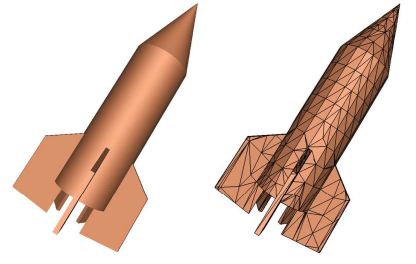
\includegraphics[width=\textwidth]{Images/TriangleMesh.png}
	\caption{Example of a triangle mesh, the most commonly used method for representing 3D objects in computer graphics. Source: \cite{Mesh}.}
	\label{fig:trianglemesh}
\end{figure}
\FloatBarrier
\noindent
\subsubsection{Neural Radiance Fields}
One popular approach to addressing these challenges is Neural Radiance Fields (NeRF) \parencite{Nerf}. This method employs a neural network to learn a mapping from 3D position and viewing direction to a density and an RGB color. The network is trained on a video or a collection of images, allowing it to reconstruct a scene by learning the underlying volumetric representation. During rendering, a ray is cast through each pixel of the screen, and multiple points along the ray are sampled. The neural network takes the position of each point and the viewing direction of the ray as input, producing color and density values. These outputs are then aggregated to compute the final color of the pixel, enabling the generation of photorealistic scenes without the need for manually crafted 3D models (see Figure~\ref{fig:nerf}). However, due to the necessity of querying the neural network multiple times per pixel, this approach is computationally expensive and not suitable for real-time rendering.
\begin{figure}[h!]
	\centering
	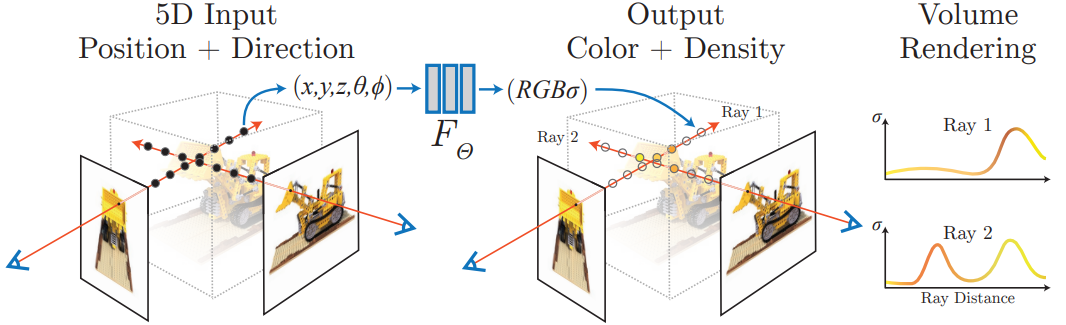
\includegraphics[width=\textwidth]{Images/Nerf.png}
	\caption{Rendering a scene using Neural Radiance Fields. Source: \cite{Nerf}.}
	\label{fig:nerf}
\end{figure}
\subsubsection{Gaussian Splatting}
In 2023, a method was introduced that retained the advantages of Neural Radiance Fields, while achieving real-time processing: Gaussian Splatting \parencite{OriginalSplatting}. Like Neural Radiance Fields, Gaussian Splatting uses a video or a collection of images as input to automatically generate the 3D scene data. However, rather than relying on a neural network to represent the data, the scene is represented as a collection of numerous small 3D Gaussians (see Figure~\ref{fig:Form}).
\begin{figure}[h!]
	\centering
	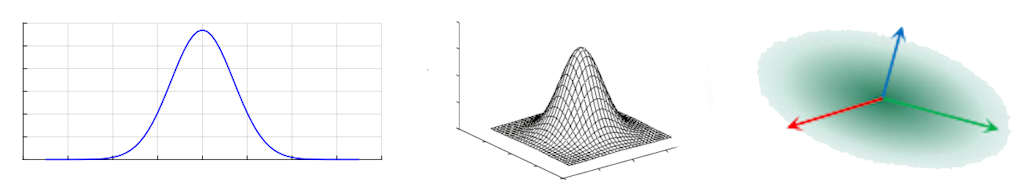
\includegraphics[width=\textwidth]{Images/GaussianForm.png}
	\caption{Illustration of Gaussian functions in different dimensions, shown left to right: 1D Gaussian \parencite{1DGaussian}, 2D Gaussian \parencite{2DGaussian}, and 3D Gaussian \parencite{3DGaussian}.}
	\label{fig:Form}
\end{figure}
\newpage  \noindent
Each Gaussian is defined by several attributes that determine its appearance and behavior during rendering:
\begin{itemize}
	\item 3D coordinates
	\item Opacity (transparency)
	\item Anisotropic covariance: The degree to which the Gaussian is 'stretched' along each of the three axes independently
	\item Spherical Harmonics: The color of the Gaussian, which varies depending on the viewing angle
\end{itemize}
The key advantage of this approach is the way the scene is rendered. Instead of relying on rays or neural networks, which are computationally expensive, Gaussian Splatting leverages a rasterization technique. In this process, the 3D Gaussians are projected directly onto the 2D screen space, where they are rendered as small, disk-like splats. These splats are then blended together based on their spatial overlap, opacity, and color attributes.\\
Furthermore, state-of-the-art triangle mesh rendering also relies on rasterization, meaning that this approach already benefits from many well-established optimizations in graphics hardware. These optimizations, including efficient handling of spatial data and parallel processing, are directly applicable to Gaussian Splatting. By utilizing the same rendering pipeline, Gaussian Splatting can leverage these optimizations for further efficiency gains, making it an ideal choice for real-time rendering applications.
\subsection{Unity Extension}
\label{sec:pipeline_overview}
\subsubsection{Introduction}
When adapting this technique to interactive applications —such as games—several engines come to mind, including Unity, Godot, and Unreal Engine. Among these, Unity was chosen due to prior experience with the engine. Additionally, a widely referenced GitHub project \parencite{Aras} implementing Gaussian Splatting in Unity provides a strong foundation for further research. This project stands out not only for its recognition within the community \parencite{ArasRecc1,ArasRecc2}, but also for its developer, Aras Pranckevičius, a former Unity engineer with 15 years of experience working on the engine. His expertise suggests that the rendering pipeline adaptations are both well-optimized and efficiently integrated, making this implementation a suitable choice for exploration and development.
\\\\
Before examining the objectives of this thesis and the adaptations made to the selected implementation, it is essential to first outline the relevant aspects of its rendering pipeline. The discussion will focus solely on components that directly influence the rendering process. Certain aspects, such as the compression and storage of Gaussian Splats in files, among others, fall outside the scope of this explanation and will not be covered.
\subsubsection{Adding a Gaussian Splat to the Scene}
The selected project does not implement the training of Gaussian Splats but instead relies on pretrained models obtained from an external source. These models are not used in their original format; rather, the project includes a Unity Editor extension that converts them into a more efficient and compressed representation (see Figure~\ref{fig:creator}). As previously mentioned, the specifics of this compression process have minimal impact on rendering and will therefore not be discussed in detail. Once the compressed asset is generated, the user must manually create a new empty GameObject and attach the \texttt{GaussianSplatRenderer} script to it. This script includes a field labeled Asset, into which the compressed asset must be assigned. Upon doing so, the Gaussian Splat appears in the scene. Like any GameObject in Unity, it can be translated, rotated, and scaled. This process can be repeated to instantiate multiple Gaussian Splats within the same scene.
\begin{figure}[h!]
	\centering
	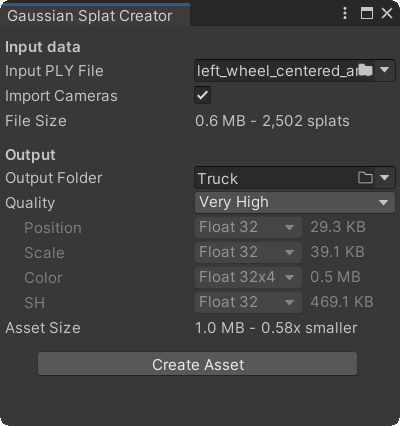
\includegraphics[width=0.5\textwidth]{Images/SplatCreator.png}
	\caption{The Unity Editor extension included in the project for converting PLY files into the required compressed format.}
	\label{fig:creator}
\end{figure}
\subsubsection{Initializing the Rendering Process: The Role of \texttt{OnEnable}}
When no GameObjects with an attached \texttt{GaussianSplatRenderer} script are present, the renderer follows the standard rendering pipeline. However, once such a GameObject is enabled, its \texttt{OnEnable} method is executed, performing several initialization tasks. The method is outlined in the following code fragment:
\lstset{style=sharpc}
\begin{lstlisting}[tabsize=2,caption=\texttt{onEnable} of \texttt{GaussianSplatRenderer}, label=code:rendereronenable,breaklines=true,breakatwhitespace=true,basicstyle=\ttfamily\footnotesize]
public void OnEnable()
{
  // Check if necessary shaders and compute shaders are available

	// Initialize materials (details omitted, see later)
	
	// Initialize the sorter
	
	GaussianSplatRenderSystem.instance.RegisterSplat(this);
	
	// Initialize all the graphics buffers
}
\end{lstlisting}
As demonstrated in the code segment, the \texttt{OnEnable} method calls the \linebreak\texttt{RegisterSplat} function of \texttt{GaussianSplatRenderSystem}, a singleton class. This class plays a pivotal role in managing the multiple \linebreak\texttt{GaussianSplatRenderer} objects within the scene and is responsible for executing the changes that modify the rendering process. The implementation of the \texttt{RegisterSplat} function is as follows
\begin{lstlisting}[tabsize=2,caption=\texttt{RegisterSplat} of \texttt{GaussianSplatRenderSystem}, label=code:systemregister,breaklines=true,breakatwhitespace=true,basicstyle=\ttfamily\footnotesize]
public void RegisterSplat(GaussianSplatRenderer r)
{
	if (m_Splats.Count == 0)
	{
		if (GraphicsSettings.currentRenderPipeline == null)
		Camera.onPreCull += OnPreCullCamera;
	}
	m_Splats.Add(r, new MaterialPropertyBlock());
}
\end{lstlisting}
The \texttt{GaussianSplatRenderSystem} maintains a dictionary of all enabled \linebreak\texttt{GaussianSplatRenderer} objects. When this function is invoked, and no other \texttt{GaussianSplatRenderer} are registered, the method subscribes to the \texttt{Camera.onPreCull} event, linking it to the \texttt{OnPreCullCamera} method.\\
When a \texttt{GaussianSplatRenderer} is disabled, it clears all associated buffers and materials, removes the object from the internal dictionary, and unsubscribes from the \texttt{onPreCull} event when the last \texttt{GaussianSplatRenderer} is removed, effectively managing resources and maintaining system efficiency.
\subsubsection{The Rendering Pipeline}
Each frame, the Unity engine performs culling before rendering the scene, determining which objects lie within the camera’s view and should be processed for rendering. Since splats may appear outside of the camera’s view, the moment just prior to culling is an optimal point at which to prepare these splats and enqueue their draw procedure in the command buffer for execution during the rendering stage. That moment is when \texttt{onPreCull} calls are made.\\
As previously mentioned, when the first \texttt{GaussianSplatRenderer} is enabled, the \texttt{OnPreCullCamera} function is linked to \texttt{onPreCull}. The implementation of this function is as follows:
\begin{lstlisting}[tabsize=2,caption=\texttt{OnPreCullCamera} of \texttt{GaussianSplatRenderSystem}, label=code:systemprecull,breaklines=true,breakatwhitespace=true,basicstyle=\ttfamily\footnotesize]
void OnPreCullCamera(Camera cam)
{
	if (!GatherSplatsForCamera(cam))
	return;
	
	InitialClearCmdBuffer(cam);
	
	m_CommandBuffer.GetTemporaryRT( GaussianSplatRenderer.Props.GaussianSplatRT, -1, -1, 0, FilterMode.Point, GraphicsFormat.R16G16B16A16_SFloat);
	m_CommandBuffer.SetRenderTarget( GaussianSplatRenderer.Props.GaussianSplatRT, BuiltinRenderTextureType.CurrentActive);
	m_CommandBuffer.ClearRenderTarget(RTClearFlags.Color, new Color(0, 0, 0, 0), 0, 0);
	
	// add sorting, view calc and drawing commands for each splat object
	Material matComposite = SortAndRenderSplats(cam, m_CommandBuffer);
	
	// compose
	m_CommandBuffer.BeginSample(s_ProfCompose);
	m_CommandBuffer.SetRenderTarget( BuiltinRenderTextureType.CameraTarget);
	m_CommandBuffer.DrawProcedural(Matrix4x4.identity, matComposite, 0, MeshTopology.Triangles, 3, 1);
	m_CommandBuffer.EndSample(s_ProfCompose);
	m_CommandBuffer.ReleaseTemporaryRT( GaussianSplatRenderer.Props.GaussianSplatRT);
}
\end{lstlisting}
This function performs 5 key operations:
\begin{itemize}
	\item \texttt{GatherSplatsForCamera}: This function first iterates over all key-value pairs in \texttt{m\textunderscore Splats} and selects those that have a valid compressed asset assigned, storing them in the list \texttt{m\textunderscore ActiveSplats}. Subsequently, this list is sorted based on the depth of each entry’s transform in the camera’s coordinate space. The implementation of this function will be presented later.
	\item \texttt{InitialClearCmdBuffer}: This function initializes and clears a command buffer, \texttt{m\textunderscore CommandBuffer}, before attaching it to the camera. By doing so, draw commands, which are created in later parts of the code, can be enqueued into this buffer. Each draw command ensures execution during the later rendering process if it is not culled.
	\item The function creates a temporary render target, \texttt{GaussianSplatRT}, sets it as the active render target, and clears it. Consequently, any draw calls issued before the render target is switched again will render to this temporary target rather than directly to the camera’s output.
	\item \texttt{SortAndRenderSplats}: This function is responsible for the main calculations. It processes all collected splats and enqueues the necessary draw commands to render them into \texttt{GaussianSplatRT}. The implementation of this function will be presented later.
	\item  The render target is reset to the camera’s primary output, after which a \texttt{DrawProcedural} call is issued using a designated material. This material is associated with a shader that generates a single triangle that covers the entire screen in its vertex shader. The fragment shader subsequently reads data from \texttt{GaussianSplatRT} and applies gamma correction. This \texttt{DrawProcedural} call enqueues the rendering of this full-screen triangle, ensuring that the Gaussian Splats are correctly displayed in the final rendered image.
\end{itemize}
To fully understand what gets rendered to the screen, it is essential to take a close look at \texttt{SortAndRenderSplats}:
\begin{lstlisting}[tabsize=2,caption=\texttt{SortAndRenderSplats} of \texttt{GaussianSplatRenderSystem}, label=code:systemsortrender,breaklines=true,breakatwhitespace=true,basicstyle=\ttfamily\footnotesize]
public Material SortAndRenderSplats(Camera cam, CommandBuffer cmb)
{
	Material matComposite = null;
	foreach (var kvp in m_ActiveSplats)
	{
		var gs = kvp.Item1;
		matComposite = gs.m_MatComposite;
		var mpb = kvp.Item2;
		
		// sort
		var matrix = gs.transform.localToWorldMatrix;
		if (gs.m_FrameCounter % gs.m_SortNthFrame == 0)
		gs.SortPoints(cmb, cam, matrix);
		++gs.m_FrameCounter;
		
		kvp.Item2.Clear();
		
		// [Omitted: Set some variables related to debugging]
		
		gs.SetAssetDataOnMaterial(mpb);
		mpb.SetBuffer(GaussianSplatRenderer.Props.SplatChunks, gs.m_GpuChunks);
		
		mpb.SetBuffer(GaussianSplatRenderer.Props.SplatViewData, gs.m_GpuView);
		
		mpb.SetBuffer(GaussianSplatRenderer.Props.OrderBuffer, gs.m_GpuSortKeys);
		mpb.SetFloat(GaussianSplatRenderer.Props.SplatScale, gs.m_SplatScale);
		mpb.SetFloat(GaussianSplatRenderer.Props.SplatOpacityScale, gs.m_OpacityScale);
		mpb.SetFloat(GaussianSplatRenderer.Props.SplatSize, gs.m_PointDisplaySize);
		mpb.SetInteger(GaussianSplatRenderer.Props.SHOrder, gs.m_SHOrder);
		mpb.SetInteger(GaussianSplatRenderer.Props.SHOnly, gs.m_SHOnly ? 1 : 0);
		mpb.SetInteger(GaussianSplatRenderer.Props.DisplayIndex, gs.m_RenderMode == GaussianSplatRenderer.RenderMode.DebugPointIndices ? 1 : 0);
		mpb.SetInteger(GaussianSplatRenderer.Props.DisplayChunks, gs.m_RenderMode == GaussianSplatRenderer.RenderMode.DebugChunkBounds ? 1 : 0);
		
		cmb.BeginSample(s_ProfCalcView);
		gs.CalcViewData(cmb, cam, matrix);
		cmb.EndSample(s_ProfCalcView);
		
		// [Omitted: Set some variables related to debugging]
		
		cmb.BeginSample(s_ProfDraw);
		cmb.DrawProcedural(gs.m_GpuIndexBuffer, matrix, displayMat, 0, topology, indexCount, instanceCount, mpb);
		cmb.EndSample(s_ProfDraw);
	}
	return matComposite;
}
\end{lstlisting}
This code block is extensive and encompasses multiple operations. To facilitate a clearer understanding, it will be analyzed step by step, broken down into its fundamental components. Additionally, certain sections of the code are dedicated to debugging or timing purposes, which are not essential for understanding the main rendering pipeline.\\\\
The function iterates over all \texttt{GaussianSplatRenderer} objects stored and ordered in the \texttt{m\textunderscore ActiveSplats} list by \texttt{GatherSplatsForCamera}. It is important to emphasize that within this function, all subsequent operations are performed on a single \texttt{GaussianSplatRenderer} object at a time, as each iteration of the loop processes one individual \texttt{GaussianSplatRenderer}.\\\\
At regular intervals, specifically every set number of frames, the splats undergo sorting. This operation is managed by a custom sorter class, which was initialized during the \texttt{OnEnable} method. The class implements a specialized sorting algorithm known as "Device Radix Sort," leveraging the full potential of the GPU to ensure optimal performance. According to the comments in that class, this algorithm was adapted from another GitHub project \parencite{Sorting}. As with the sorting of the \texttt{GaussianSplatRenderer} objects, the depth of each splat relative to the camera’s coordinate space is used as the key for sorting.
\\\\
Similar to the final \texttt{DrawProcedural} invocation of the previous function, a material shader is employed at the end of each iteration of the loop to render the splats. Many of the operations within this loop are dedicated to populating graphics buffers with the necessary data for these shader computations. The most significant step in this process is the invocation of \texttt{CalcViewData}, which dispatches splat-related information to a compute shader. This compute shader determines the screen-space position of each splat using the object's transform matrix, the \texttt{cam.worldToCameraMatrix}, and the \texttt{cam.projectionMatrix}. Additionally, it calculates its independent horizontal and vertical extents, and derives its color and transparency based on the viewing angle and spherical harmonics. The computed results are then stored in a graphics buffer for subsequent use. \\\\
Finally, \texttt{DrawProcedural} is called, enqueueing the rendering of this data for execution later in the rendering pipeline. This rendering step is also performed using a material shader, distinct from the shader used in \texttt{OnPreCullCamera}. Each splat is represented as two triangles, with the vertex shader transforming the computed screen position and stretch extents into appropriate triangle coordinates.
\\\\
As a brief reminder, as stated earlier, this \texttt{DrawProcedural} invocation does not render directly to the camera’s output but instead to the temporary render target \texttt{GaussianSplatRT}. Additionally, due to the sorting performed at the beginning of the loop, splats farther from the camera are rendered before those closer to it, ensuring correct per-object rendering order.\\\\
With these steps described, the overall structure of the rendering pipeline for the Gaussian Splats becomes clear. The coordination between sorting, compute shaders, and material shaders ensures that the splats are accurately positioned, stretched, and rendered according to the camera’s view.
\section{Part 1: Correcting the Rendering Order}    
\subsection{Introduction}   
At the outset of this research, no specific focus or predefined problem statement had been established. The initial objective was exploratory in nature: to experiment with the existing Unity extension and investigate the process of importing and animating a Gaussian Splat within the engine.\\
Throughout this exploratory process, particular attention was given to identifying tasks that were difficult to perform, as well as outputs that appeared incorrect or inconsistent. These observations served as the basis for defining the core focus areas of the thesis.
\subsection{Preparing the scene}
To initiate this phase of the research, it was necessary to select a suitable pre-trained Gaussian Splat model. Ideally, the chosen model would consist of multiple visually distinct segments, making it intuitive and practical for experimentation with segmentation and animation. The primary models considered were those released by the authors of the original Gaussian Splatting paper. Among them, the Kitchen scene includes a small LEGO bulldozer—an object that is compact, easily recognizable, and composed of several clearly separable parts (see Figure~\ref{fig:kitchen}). These characteristics made it an ideal candidate for the intended use case.
\begin{figure}[h!]
	\centering
	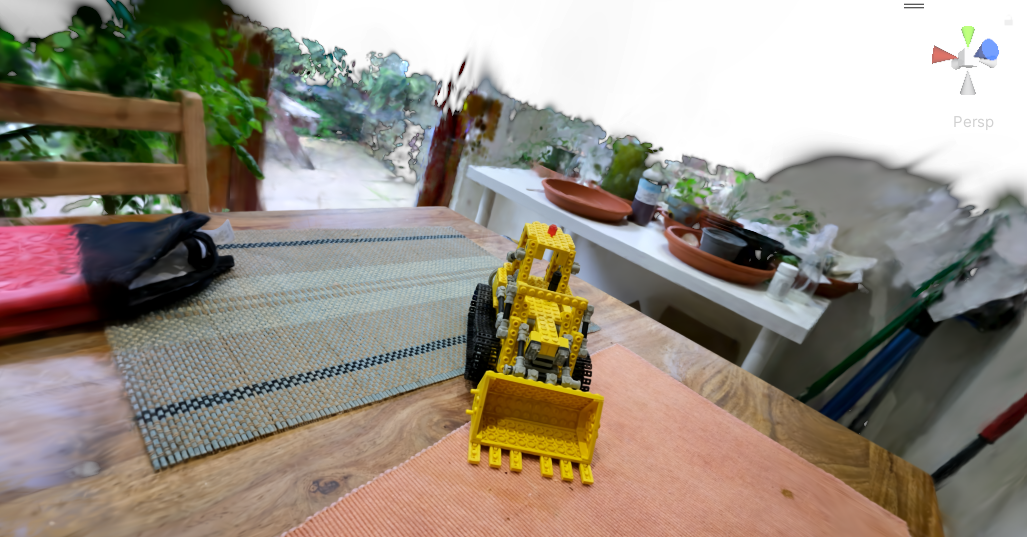
\includegraphics[width=\textwidth]{Images/Kitchen.png}
	\caption{The Kitchen scene from the official Gaussian Splatting dataset, featuring a small LEGO bulldozer. This object was selected for its compact structure and clearly defined components, making it well-suited for segmentation and animation experiments.}
	\label{fig:kitchen}
\end{figure}
\FloatBarrier
\noindent
For these purposes, only the LEGO bulldozer is required, and not the entire scene. Fortunately, the Unity extension being used includes a tool designed specifically for this type of task: cutouts. Within the GaussianSplatRenderer component of the relevant GameObject in the Unity Editor, a cutout can be added to the Gaussian Splat. This tool creates a cutout GameObject (either a box or an ellipsoid) as a child of the selected object. The cutout can be translated, rotated, and scaled like any other GameObject. Any splats of the selected object outside of the cutout are excluded from rendering. Additionally, there is an invert option that reverses the effect, making only the splats within the cutout invisible. A button allows the Gaussian Splat to be saved as a PLY file, accounting for all cutout modifications. This functionality was used to generate a PLY file and associated asset containing only the bulldozer, omitting the rest of the scene (see Figure~\ref{fig:wholetruck}).
\begin{figure}[h!]
	\centering
	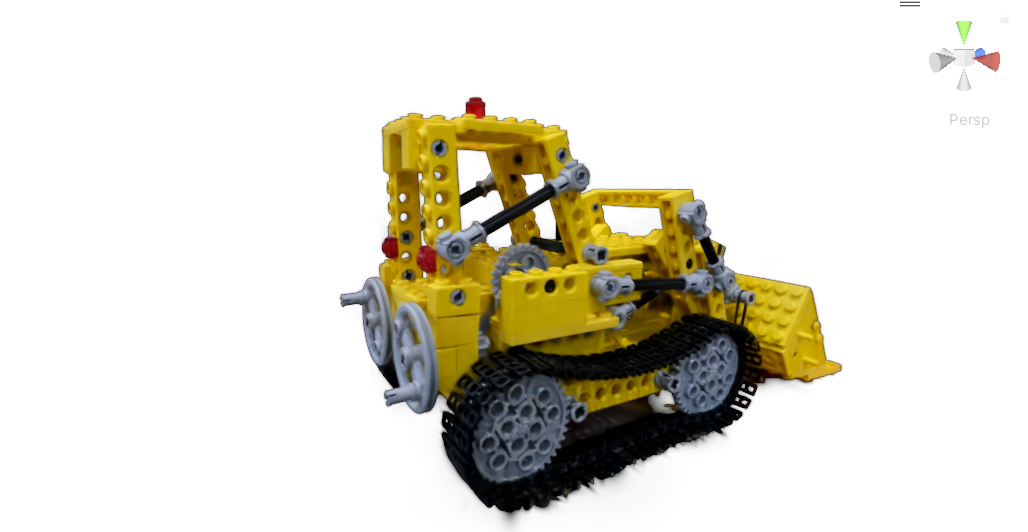
\includegraphics[width=\textwidth]{Images/WholeTruck.png}
	\caption{The LEGO bulldozer extracted from the Kitchen scene using the cutout tool of the Unity extension for Gaussian splatting. This tool isolates the bulldozer by excluding all other parts of the scene.}
	\label{fig:wholetruck}
\end{figure}
\FloatBarrier
\noindent
\subsection{Animating a segment}
To animate the LEGO bulldozer, the next step was to segment it into multiple parts, with each part represented as a separate GameObject and parented to the main bulldozer GameObject. Instead of segmenting the entire model at once, segmentation began with a single part to test the process. The first part selected for segmentation was one of the wheels at the back of the bulldozer. Using the cutout tool, a cutout was created that perfectly covered the wheel, allowing for the generation of a PLY file containing only the wheel. To isolate the bulldozer without the wheel, the same cutout was applied with the invert option enabled. However, when the separate wheel GameObject was rendered, it appeared behind the rest of the bulldozer, resulting in an unexpected rendering error (see Figure~\ref{fig:firstwheel}).
\begin{figure}[h!]
	\centering
	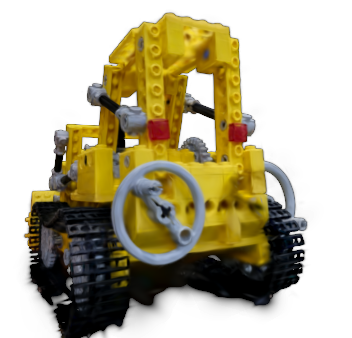
\includegraphics[width=0.5\textwidth]{Images/first_wheel.png}
	\caption{A rendering error when loading the separate wheel-GameObject.}
	\label{fig:firstwheel}
\end{figure}
\FloatBarrier
\noindent
This issue can be mitigated by adjusting the z-value of the wheel GameObject’s position to $0.001$. Nonetheless, the need for this workaround already indicates that something is fundamentally wrong with the rendering process.
\\\\
The next objective was to rotate the wheel around its own axis. However, this revealed a new challenge: the center of the wheel’s GameObject was inherited from the original full scene and therefore located far from the actual center of the wheel. In addition, the existing rotation axes were misaligned with the intended axes of rotation (see Figure~\ref{fig:wheel_center}).
\begin{figure}[h!]
	\centering
	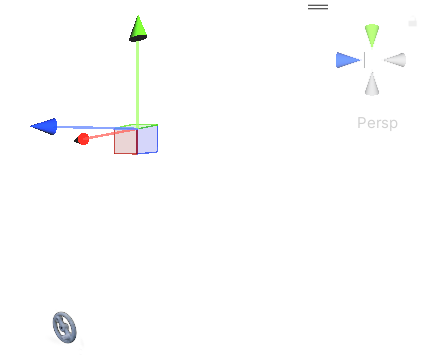
\includegraphics[width=0.5\textwidth]{Images/wheel_center.png}
	\caption{The center of the wheel’s GameObject is positioned far from the geometric center of the wheel, with misaligned axes of rotation. This misalignment complicates direct rotation around the wheel’s local axis.}
	\label{fig:wheel_center}
\end{figure}
\FloatBarrier
\noindent
A seemingly straightforward solution is implemented to achieve what appears to be the desired result. A small, distinctively colored cube is created and designated as the parent of the wheel GameObject. The wheel is then repositioned and rotated relative to the cube so that its center aligns with the center of the cube and its plane is parallel to the cube’s axes (see Figure~\ref{fig:wheel_cube}). Once this alignment is achieved, the cube is made invisible. By rotating the parent, the wheel now rotates correctly around the intended axis. The same procedure was applied to the base of the bulldozer to achieve similar control.
\begin{figure}[h!]
	\centering
	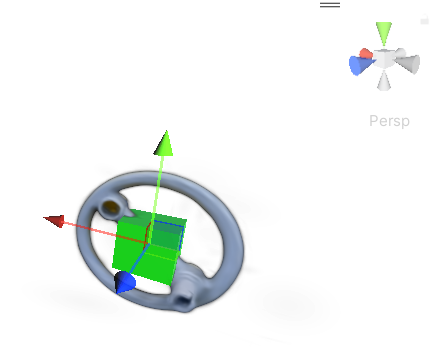
\includegraphics[width=0.5\textwidth]{Images/wheel_cube.png}
	\caption{A cube GameObject is assigned as the parent of the wheel GameObject. The wheel is repositioned and rotated so that its center and axes align with those of the cube. This configuration enables rotation around the intended axis.}
	\label{fig:wheel_cube}
\end{figure}
\FloatBarrier
\noindent
A simple animation was created using Unity’s built-in Animation feature to rotate the wheel around its axis. However, this exposed a flaw in the proposed solution: the wheel exhibited flickering during rotation, appearing in front of the bulldozer at certain angles and behind it at others (see Figure~\ref{fig:wheel_rotations}).
\\
Further inspection revealed the underlying cause: rotating the wheel around the new axis also rotates the center of the Gaussian Splat itself—still located at the center of the original full scene—around that axis. Since the per-GameObject renderer relies on this center point to determine the rendering order based on its depth to the camera, any displacement of the center could lead to a different rendering order. Consequently, an alternative solution was required to prevent the center from moving during rotation.
\begin{figure}[h!]
	\centering
	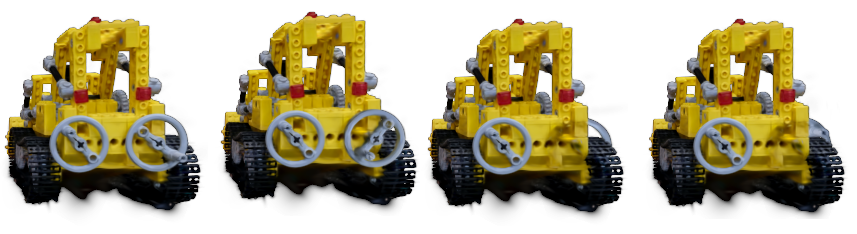
\includegraphics[width=\textwidth]{Images/wheel_rotations.png}
	\caption{Visualization of the rendering issue caused by rotation around its axis. The same wheel is shown at 0°, 90°, 180°, and 270° of rotation. Depending on the rotation angle, the wheel is rendered either behind or in front of the bulldozer due to improper depth sorting based on the rotated center of the Gaussian Splat.}
	\label{fig:wheel_rotations}
\end{figure}
\FloatBarrier
\noindent
A viable approach to eliminating this visual artifact involves aligning the origin of the Gaussian Splat with the geometric center of the wheel. This requires modifying the underlying splat data in the corresponding .ply file. To achieve this, a small Python script was developed to automatically adjust the position values of each splat.
\\
Initially, it seemed straightforward to have the script infer the desired center point automatically. Two potential approaches were implemented: calculating the average of the position values of all splats, and calculating the midpoint between the minimum and maximum position values along each axis. However, testing revealed that both methods resulted in a center point that was slightly offset, leading to imperfect alignment (see Figure~\ref{fig:left_av}). While other automatic methods, such as taking the size of the splats into account, could have been explored, they were not pursued. Instead, the decision was made to allow the user to manually input an offset value for greater control, particularly in cases where complex and irregular shapes may have a "desired" center that is difficult to compute automatically. The desired offset can be determined by applying the earlier alignment procedure with the cube and copying the position values of the wheel GameObject relative to its parent. The Python function solely modifies the center point of the GameObject, leaving the alignment of the axes unchanged, which is still achieved through the cube method. The most relevant part of the resulting Python script is provided below. The plyfile library \parencite{Plyfile} was used to load, edit and store the splat data:
\begin{lstlisting}[tabsize=2,caption=Three potential functions for recentering the Gaussian Splat. The desired function is called on each of the three axes., label=code:re_center,breaklines=true,breakatwhitespace=true,basicstyle=\ttfamily\footnotesize]
def recenter_axis_average(ply_content, axis):
	axis_poses = ply_content.elements[0].data[axis]
	axis_avg = axis_poses.mean()
	axis_poses -= axis_avg

def recenter_axis_box(ply_content, axis):
	axis_poses = ply_content.elements[0].data[axis]
	axis_middle = (axis_poses.max()+axis_poses.min())/2
	axis_poses -= axis_middle

def recenter_axis_offset(ply_content, axis, offset):
	axis_poses = ply_content.elements[0].data[axis]
	axis_poses += offset

\end{lstlisting}
\begin{figure}[h!]
	\centering
	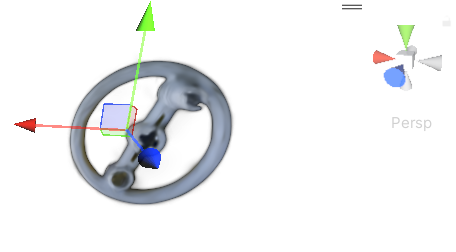
\includegraphics[width=0.5\textwidth]{Images/left_wheel_av.png}
	\caption{Automatically recentering based on the average of the position values results in a slight offset. Recentering using the midpoint of the bounding box yields a similar misalignment.}
	\label{fig:left_av}
\end{figure}
\FloatBarrier
\noindent
\subsection{Moving the camera}
The wheel now both renders and rotates as intended, but these results were observed under an unambiguous camera perspective. Once the camera was moved or rotated, it became apparent that the rendering order had another issue. Specifically, rotating the camera altered the rendering order, while translating the camera had no effect. This behavior is the opposite of what one would expect for correct depth-based rendering. To better illustrate this issue—and to further validate the solution from the previous step—a second wheel was segmented into its own GameObject, following the same procedure described earlier (see Figure~\ref{fig:camera_change}).
\begin{figure}[h!]
	\centering
	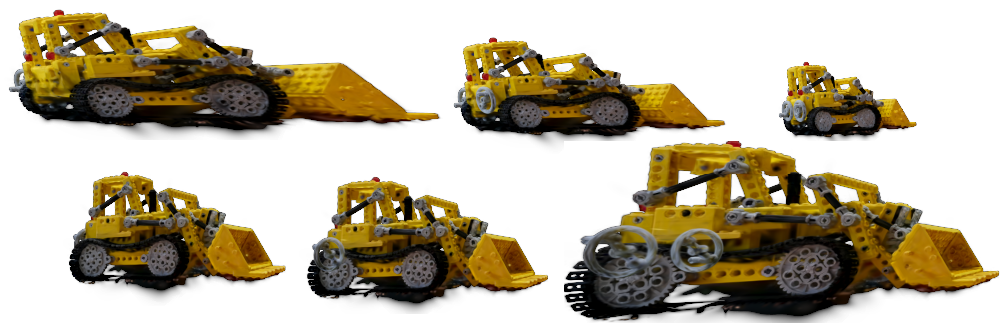
\includegraphics[width=\textwidth]{Images/camera_order.png}
	\caption{Demonstration of incorrect rendering order under camera transformation. Each column corresponds to a fixed camera rotation, while each row corresponds to a fixed camera position. The observed rendering order remains the same across rows within each column, indicating that the order is determined solely by camera rotation. Correct behavior would require the rendering order to change across rows (i.e., with camera position).}
	\label{fig:camera_change}
\end{figure}
\FloatBarrier
\noindent
It becomes evident that the problem lies within the renderer itself; therefore, adjusting the GameObjects or the splats alone cannot provide a solution. To identify the root cause, a closer examination of the Gaussian Splat rendering process is necessary. A general overview of the pipeline was provided earlier in this thesis. In summary:\\
The renderer maintains a data structure that holds all enabled Gaussian Splats. First, it sorts these GameObjects based on the depth of each entry’s transform in the camera’s coordinate space. Then, for each GameObject, the individual splats are sorted, and the screen position and shape of each are computed and rendered.\\
The flaw is immediately apparent in this summary: the method of sorting the GameObjects.\\
When the camera is translated (without rotation), the relative depth of each GameObject remains unchanged. That is, if the depth of one GameObject increases by a certain amount, all others increase by the same amount, leaving the rendering order unaffected.\\
Conversely, when the camera is rotated, the depth of each GameObject relative to the camera’s plane changes differently, resulting in a new rendering order.\\
The code of this functionality can be found below:
\begin{lstlisting}[tabsize=2,caption=The sort key used to determine the rendering order, label=code:sort_original,breaklines=true,breakatwhitespace=true,basicstyle=\ttfamily\footnotesize]
var trA = a.Item1.transform;
var trB = b.Item1.transform;
var posA = camTr.InverseTransformPoint(trA.position);
var posB = camTr.InverseTransformPoint(trB.position);
return posA.z.CompareTo(posB.z);
\end{lstlisting}
To resolve this, a different metric is required for sorting the GameObjects. Using the Euclidean distance to the camera itself satisfies the requirements. When the camera is translated, each GameObject’s distance to the camera changes independently, ensuring the rendering order updates correctly. When the camera is rotated, the distances remain unchanged, so the rendering order is preserved. This new sorting method thus addresses the core issue.\\
It is also worth noting that only the relative distances between GameObjects matter for determining the correct rendering order. This means that computing the exact Euclidean distance—including taking the square root of the squared distance—is not required. Instead, the squared distance can be used directly for sorting, as it preserves the same relative ordering. This approach avoids unnecessary square root calculations, improving efficiency without affecting correctness.
The new code can be found below:
\begin{lstlisting}[tabsize=2,caption=The newly implemented sort key to determine the rendering order, label=code:sort_pos,breaklines=true,breakatwhitespace=true,basicstyle=\ttfamily\footnotesize]
var trA = a.Item1.transform;
var trB = b.Item1.transform;
Vector3 APos = trA.position;
Vector3 BPos = trB.position;
float sqrDistanceA = (camPos - APos).sqrMagnitude;
float sqrDistanceB = (camPos - BPos).sqrMagnitude;
return sqrDistanceA.CompareTo(sqrDistanceB);
\end{lstlisting}
The new behavior is significantly closer to the expected result. In most camera positions and rotations, the body and wheels now render in the correct order. However, certain edge cases remain where the rendering is still incorrect (see Figure~\ref{fig:wheel_almost}).
\begin{figure}[h!]
	\centering
	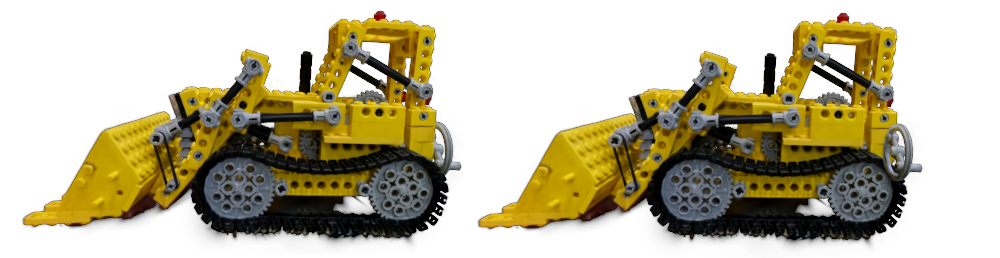
\includegraphics[width=\textwidth]{Images/wheel_almost.png}
	\caption{When the wheel should be rendered behind the bulldozer, but the camera is positioned near the threshold where the rendering order switches, the wheel is incorrectly rendered in front of the bulldozer. The left and right images have identical camera rotation, with only a minimal difference in camera position.}
	\label{fig:wheel_almost}
\end{figure}
\FloatBarrier
\noindent
The core of the problem is that the renderer compares only the center points of each GameObject to determine depth order. In this scenario, the center of the bulldozer is located far from the region where overlap with the wheel actually occurs. While this comparison yields correct results from many viewing positions, it fails when the camera is positioned near or between the two center points, where the relative depth becomes ambiguous or misleading.\\
For nested GameObjects, there is typically a logical connection point—namely, the position where the child segment physically attaches to the parent. Ideally, the depth comparison would be made between this connection point and the center of the child segment (the wheel, in this case). However, accurately determining the exact location of this connection point is non-trivial.\\
A practical alternative achieves a similar effect: introducing a pseudo-connection point along the line connecting the centers of the two GameObjects. This point is placed much closer to the center of the child than to that of the parent. By comparing this pseudo-connection point to the center of the child, a more stable and intuitive depth ordering can be achieved. This approach provides a better representation of the true spatial relationship between the two objects and ensures that the camera can no longer be positioned between the child’s center and the new pseudo-connection point, thereby eliminating the ambiguous scenarios that previously caused incorrect rendering order. The code is provided below. Note that the method for determining the parent-child relationship is structured in this particular way due to the earlier alignment procedure, where each Gaussian Splat was made a child of an invisible cube to align the rotation axes.
\begin{lstlisting}[tabsize=2,caption=The final implemention of the sort key, label=code:sort_ratio,breaklines=true,breakatwhitespace=true,basicstyle=\ttfamily\footnotesize]
Vector3 APos = trA.position;
Vector3 BPos = trB.position;
float ratio = 0.999f;
if (trA.parent == trB.parent.parent)
{
	APos = APos * (1 - ratio) + BPos * ratio;
}else if (trB.parent == trA.parent.parent)
{
	BPos = BPos * (1 - ratio) + APos * ratio;
}

float sqrDistanceA = (camPos - APos).sqrMagnitude;
float sqrDistanceB = (camPos - BPos).sqrMagnitude;

return sqrDistanceA.CompareTo(sqrDistanceB);
\end{lstlisting}
Finally, the wheels render as expected, as illustrated in Figure~\ref{fig:wheel_almost}.
\begin{figure}[h!]
	\centering
	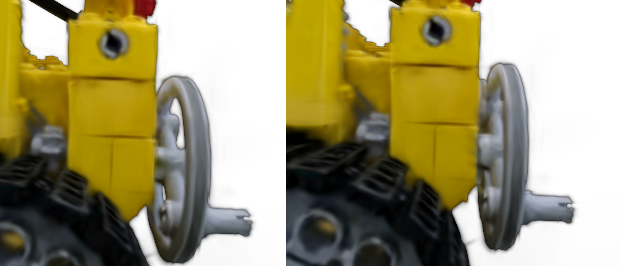
\includegraphics[width=\textwidth]{Images/sort_done.png}
	\caption{The camera is positioned at the critical point where the wheel should transition from being rendered behind the bulldozer to being rendered in front of it. The left and right images have identical camera rotations, with only a minimal change in camera position. As shown, the wheel now renders correctly across this boundary case.}
	\label{fig:wheel_done}
\end{figure}
\FloatBarrier
\noindent
\subsection{Global per-splat sorting}
With the basic subsegments now rendering correctly, the question arose whether to continue pursuing deeper improvements in this area or to shift focus toward other stages of the animation process that might require further research. It is important to recall that the overarching aim of this thesis is to identify and address the most significant challenges or errors across the entire pipeline.\\
To evaluate whether the current rendering solution was adequate enough to justify moving on, more complex subsegments were isolated from the bulldozer model. In particular, the arm and its claw were selected for testing. The arm presents a notably more challenging case, as it wraps around the bulldozer, resulting in certain parts that must be rendered in front of the bulldozer, while others need to appear behind it (see Figure~\ref{fig:arm}).
\begin{figure}[h!]
	\centering
	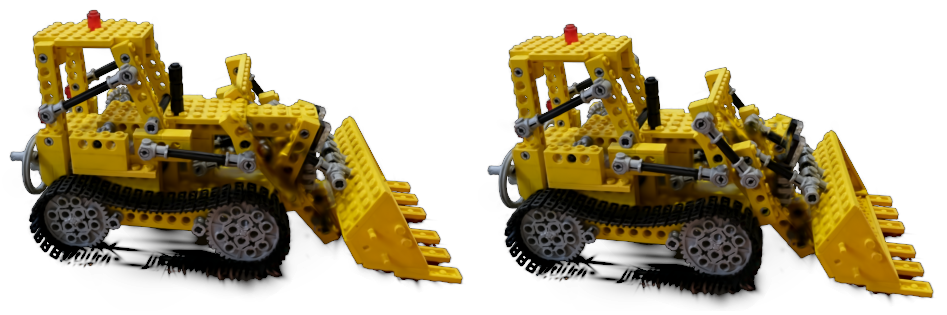
\includegraphics[width=\textwidth]{Images/arm.png}
	\caption{Regardless of the camera position, a visual artifact always occurs. When the arm is rendered behind the bulldozer (left), significant portions of its joints are lost. Conversely, when the bulldozer is rendered behind the arm, its front section is improperly occluded (right). The two images were captured with identical camera rotations and only a small difference in camera position.}
	\label{fig:arm}
\end{figure}
\FloatBarrier
\noindent
After careful evaluation, it was concluded that the visual artifacts introduced by the current rendering approach are too disruptive to be ignored. This is particularly evident in interactive environments, such as games, where objects are frequently in motion and subject to continuous rotation. In such contexts, the visual inconsistencies become highly noticeable, making it worthwhile to invest further effort into resolving the issue.
\\\\
Up to this point, most of the proposed solutions have relied on workaround-based approaches—methods that attempt to circumvent the core issue rather than address it directly. While such strategies have proven effective for simpler configurations, they fall short when applied to more complex geometries. The fundamental limitation lies in the renderer’s architecture: it operates on a per-GameObject basis, where entire GameObjects are first sorted relative to the camera, and only then are the splats within each GameObject sorted and rendered. This structure inherently fails in cases where different parts of a child object must appear both in front of and behind its parent. No amount of adjustment or approximation can resolve this limitation cleanly. A proper solution therefore requires a shift from per-GameObject sorting to fully global per-splat sorting—ensuring that every splat is sorted and rendered based solely on its position in space, regardless of GameObject hierarchy.\\\\
Since the core rendering system is now being modified directly, it is essential to first understand how the existing renderer functions. A detailed explanation of the current rendering pipeline is provided in Section~\ref{sec:pipeline_overview}.
\\\\
To clearly present the implemented solution, it is helpful to begin by outlining the desired end result. The current rendering pipeline operates on a per-GameObject basis due to its underlying architecture. Each GameObject is processed independently, with its splat data prepared and stored in a separate graphics buffer. This buffer is generated by a compute shader dispatched specifically for that GameObject, since the shader requires access to the GameObject's local data and transform in order to populate the buffer correctly. Once populated, the buffer is passed to a \texttt{DrawProcedural} call to handle sorting and rendering of the splats contained within.\\
Ideally, the renderer would instead issue a single \texttt{DrawProcedural} call that processes a unified graphics buffer containing the data for all Gaussian splats in the scene. This would enable sorting and rendering on a per-splat level, thereby resolving the compositing issues observed with overlapping objects. However, constructing such a unified buffer in an efficient manner—without incurring significant runtime overhead or increased memory usage—is a non-trivial challenge.
\\\\
The proposed solution is to employ a large, global graphics buffer that consolidates the processed splat data for all objects. Rather than merging the individual per-GameObject buffers into this global buffer at the end of each computation—a process that would introduce additional complexity and runtime overhead—the system is designed so that all compute shaders write directly into the shared buffer. Specifically, the buffer stores the computed screen positions, stretching factors, and color data for the splats, just as was done in the per-GameObject buffers, but now combined into a single structure. To facilitate this, the shader must be informed of the specific location within the global buffer where its output should be written. This is accomplished by associating each \texttt{GaussianSplatRenderer} instance with an offset value that specifies its starting position in the buffer. Conveniently, a dictionary that maps \texttt{GaussianSplatRenderer} instances to metadata already exists, making it an ideal structure for storing these offsets. The size of the global buffer is dynamically determined and set to exactly match the total number of splats across all enabled \texttt{GaussianSplatRenderer} instances\\\\
To implement this global system, much of the logic previously contained within \texttt{GaussianSplatRenderer} is transferred to the \linebreak \texttt{GaussianSplatRenderSystem}, which now manages the shared global buffer. Each time a \texttt{GaussianSplatRenderer} is enabled or disabled, the system creates a new global buffer of the appropriate size, and the offsets are updated accordingly. When a new \texttt{GaussianSplatRenderer} is enabled, its offset is set to the size of the buffer prior to its addition, effectively placing its data at the end. When a \texttt{GaussianSplatRenderer} is disabled, the system accounts for the possibility that the removed splats are positioned anywhere within the buffer. To maintain a contiguous structure, the offsets of all \texttt{GaussianSplatRenderer} instances whose offsets are greater than that of the disabled segment are decreased by the number of splats in the disabled segment. This ensures that the global buffer remains correctly partitioned at all times. The code is provided below. Note that this approach does increase complexity, but importantly, this complexity is incurred only when a \texttt{GaussianSplatRenderer} is enabled or disabled, rather than every frame. If such events occur frequently, the new pipeline could indeed introduce additional performance overhead. However, this trade-off is limited to the frequency of structural changes in the scene, and its impact should be considered in the context of the specific application’s dynamics.
\begin{lstlisting}[tabsize=2,caption=New RegisterSplat and UnregisterSplat, label=code:register,breaklines=true,breakatwhitespace=true,basicstyle=\ttfamily\footnotesize]
public void RegisterSplat(GaussianSplatRenderer r)
{
	if (m_Splats.Count == 0)
	{
		m_FrameCounter = 0;
		if (m_CSSplatUtilities == null)
			m_CSSplatUtilities = r.m_CSSplatUtilities;
		if(m_Sorter == null)
			m_Sorter = new GpuSorting(m_CSSplatUtilities);
		if (GraphicsSettings.currentRenderPipeline == null)
			Camera.onPreCull += OnPreCullCamera;
	}
	
	m_Splats.Add(r, (new MaterialPropertyBlock(), totalSplatCount));
	
	totalSplatCount += r.asset.splatCount;
	
	m_GpuViewCombined?.Dispose();
	m_GpuViewCombined = null;
	m_GpuViewCombined = new GraphicsBuffer(GraphicsBuffer.Target.Structured, totalSplatCount, 40);
	
	// initialize sorter
}

public void UnregisterSplat(GaussianSplatRenderer r)
{
	int splatCount = r.asset.splatCount;

	if (!m_Splats.ContainsKey(r))
	return;
	
	int removedOffset = m_Splats[r].Item2;
	m_Splats.Remove(r);
	foreach (var key in m_Splats.Keys.ToList())
	{
		var value = m_Splats[key];
		if(value.Item2 > removedOffset)
		m_Splats[key] = (value.Item1,value.Item2 - splatCount);
	}
	totalSplatCount -= splatCount;
	
	m_GpuViewCombined?.Dispose();
	m_GpuViewCombined = null;
	
	if (m_Splats.Count == 0)
	{
		// clear camera buffers
		
		// clear global buffers
		
		Camera.onPreCull -= OnPreCullCamera;
	}
	else
	{
		m_GpuViewCombined = new GraphicsBuffer(GraphicsBuffer.Target.Structured, totalSplatCount, 40);
		InitSortBuffers();
	}
}
\end{lstlisting}
While all processed splat data is now consolidated in a global buffer, the sorting of splats must also be addressed. In the original implementation, sorting of splats within a \texttt{GaussianSplatRenderer} occurred prior to the calculation of screen positions, with the sort key computed via a simple, dedicated compute shader. However, in the revised system, it is not feasible to perform this sorting step before the calculation of screen positions, as the splat data only becomes available in the global buffer after these calculations are complete.\\
Fortunately, as is often the case in perspective rendering, the screen-space data is stored in homogeneous coordinates, with the depth value encoded in the fourth component. This allows the sorting to be performed directly on the fully populated global buffer, using the depth value extracted from the existing data. As a result, sorting of the global buffer can be implemented without introducing additional complexity or requiring extra data specifically to compute the sort key.\\\\
After the complete implementation of this global sorting and rendering system, with all components integrated and functioning cohesively, a fully correct rendering order has been achieved, as demonstrated in Figure~\ref{fig:finalrender}.
\begin{figure}[h!]
	\centering
	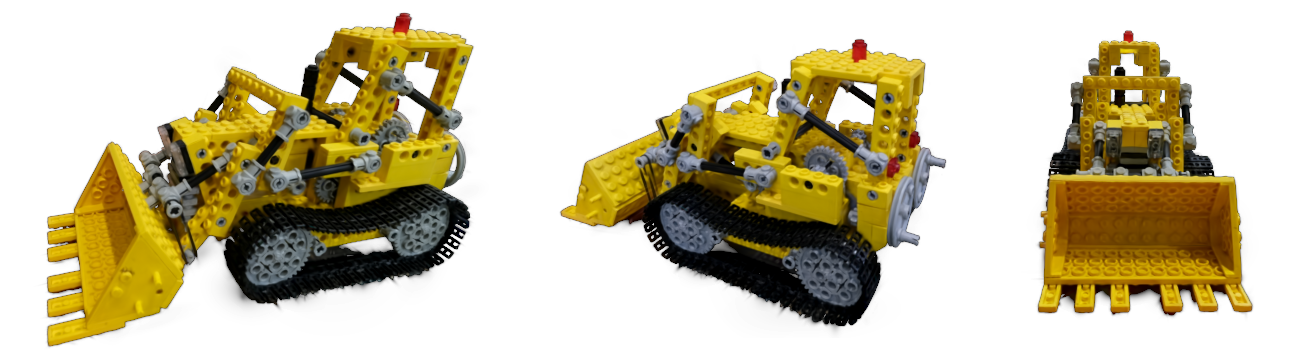
\includegraphics[width=\textwidth]{Images/finalrender.png}
	\caption{The final rendering result after implementing global per-splat sorting. Notably, both wheels at the back, the arm, and the handle are all represented as separate GameObjects, yet are rendered correctly.}
	\label{fig:finalrender}
\end{figure}
\FloatBarrier
\noindent
After further testing, a final issue was discovered, which fortunately proved to be straightforward to resolve: switching the asset assigned to a 
\linebreak 
\texttt{GaussianSplatRenderer} caused the editor to crash. This problem arose because changing the asset neither enabled nor disabled the associated GameObject, yet it still altered the number of splats represented by that object.
\\
The solution is almost trivial. Each \texttt{GaussianSplatRenderer} already stores the hash of its assigned asset within the asset itself. By also storing this hash in a local variable within the \texttt{GaussianSplatRenderer}, a straightforward comparison can be performed during each update cycle to determine whether the stored hash matches the hash currently stored in the asset. If the hashes do not match, it indicates that the asset has been changed.
\\
To resolve the resulting issues with the global buffer size and offset management, the simplest solution is to call \texttt{UnregisterSplat} followed by
\linebreak 
\texttt{RegisterSplat} for the affected \texttt{GaussianSplatRenderer}. Additionally, the number of splats associated with the current asset is stored in a local variable. This is essential because once the asset is changed, the previous splat count is no longer directly accessible, making it impossible to properly adjust the global buffer size and offsets during unregistration. To accommodate \texttt{UnregisterSplat} for this case, it can now take an optional \texttt{splatCount} argument, which by default uses the size of the current asset, as shown in the code below:
\begin{lstlisting}[tabsize=2,caption=A small adjustment to UnregisterSplat, label=code:unregister,breaklines=true,breakatwhitespace=true,basicstyle=\ttfamily\footnotesize]
public void UnregisterSplat(GaussianSplatRenderer r, int splatCount = -1)
{
	if(splatCount == -1){
		splatCount = r.asset.splatCount;
	}	
	...
}
\end{lstlisting}
\subsection{Conclusion}
The efforts detailed in this part of the thesis addressed critical rendering challenges in the Gaussian splatting pipeline. By transitioning from a per-GameObject to a fully global per-splat sorting and rendering system, the proposed solution resolved depth-ordering issues that previously resulted in visual artifacts and inconsistencies, particularly in complex scenes with overlapping splats. Through careful restructuring of the rendering architecture—including the introduction of a unified graphics buffer and adjustments to buffer management and sorting algorithms—the final implementation achieved correct and stable rendering behavior, even under dynamic camera movements and complex object hierarchies. These improvements not only enhance the visual fidelity of Gaussian splatting in Unity but also establish a robust foundation for further exploration, which will be the focus of the following section.
\section{Part 2: Hierarchical Segmentation}  
\subsection{Introduction}
While the rendering pipeline has been significantly improved, it is evident that further refinements are possible. Certain features of the original extension, such as highlighting specific splats, are no longer immediately functional due to the shift from \texttt{GaussianSplatRenderer} to the centralized \linebreak \texttt{GaussianSplatRenderSystem}. These issues, however, can be addressed by migrating the necessary functionality from the former to the latter.
\\\\
As in the previous stage of this research, it was necessary to evaluate whether pursuing these refinements would be a valuable use of time, or if efforts would be better spent addressing new challenges. This time, the circumstances differ significantly: the corrected rendering system now operates reliably across all tested scenes, with no critical issues affecting development or introducing performance bottlenecks.
\\
Given that streamlining the code and addressing residual issues represents a considerable but straightforward task, it was decided to shift the focus of this thesis toward a more substantial and technically engaging problem.  
\\\\
To determine the next focus of this thesis, it was necessary to identify the most significant remaining challenge in the entire process—from starting with a large, complete scene to arriving at individual segments that can move and rotate correctly. With the rendering errors now resolved, there were no longer any immediate errors impeding further development. The next step was to assess which aspects of the process were most cumbersome or difficult and might therefore benefit from further improvement.\\\\
Upon careful reflection, it became evident that the primary bottleneck lies in a component that this thesis has thus far only briefly mentioned: the segmentation of the splats themselves.
\\\\
As previously described, this process relies on so-called “cutouts”. In summary, cutouts are defined regions—either cuboid or ellipsoidal—that exclude either all splats inside or all splats outside of them. Extracting precise details from complex objects often requires numerous small cutouts, resulting in a cumbersome and time-consuming workflow that must be repeated for each sub-object. Moreover, this method does not permit the splitting of individual splats. This limitation has a more significant impact than one might initially expect: the interiors of objects are not captured in training images, leading to chaotic and oversized splats. When attempting to isolate a sub-segment, particularly at connection points with neighboring segments, this often results in large splats either missing or protruding awkwardly, as they cannot be bisected using this method.
\subsection{Relevant work}
Gaussian splatting is a rapidly evolving and highly promising field, with numerous research papers being published each month across a wide range of specialized topics. These include areas such as automatic meshing \parencite{automesh}, compression \parencite{compression}, physics \parencite{physics}, texturing \parencite{texture}, and many others. Unsurprisingly, segmentation has also emerged as a major area of focus within this landscape, with over 30 published papers already exploring various use cases and requirements.
\\\\
The existing literature on segmentation can broadly be categorized into two groups. The first group focuses on the fundamental task of simple segmentation, aiming to extract objects or sub-objects from larger scenes. The second group extends this concept to semantic linking, where the goal is to associate each identified object with descriptive labels or to enable object generation based on textual prompts. This latter category is often referred to as "open-vocabulary detection."
\\\\
While open-vocabulary detection techniques offer an interesting approach to user-friendly interaction, they are not the focus of this thesis. Although such methods could allow users to extract segments by describing them with natural language, incorporating these techniques would introduce a different direction for the work and require additional tools and methods. Moreover, open-vocabulary detection adds an extra layer on top of the core segmentation challenge, increasing overall complexity without directly addressing the underlying issue of precise geometric segmentation. For readers interested in exploring open-vocabulary detection methods, several representative works are available in the literature \parencite{vocab1, vocab2, vocab3}.
\\\\
Another group of important papers, though not directly relevant to the objectives of this thesis, focuses on dynamic splats \parencite{dyn1,dyn2}. These approaches extend Gaussian splatting into the temporal domain, resulting in 4D splats where the fourth dimension represents time. Effectively, they model scenes as Gaussian splats evolving over video frames. However, since this thesis operates exclusively with static 3D splats, these dynamic approaches fall outside the scope of this work.
\\\\
Finally, some papers focus on fully automatic segmentation, which requires no user input \parencite{automatic}. While these approaches are powerful, they present challenges for use in games or animation, where the segmentation of objects is not always straightforward. It is not predetermined which parts of a model should be isolated as distinct segments, and this decision can vary based on artistic or functional requirements. Therefore, it is crucial that the user retains the ability to provide guidance, enabling the segmentation tool to extract precisely the parts needed for the intended application.
\\\\
Two early and influential papers laid the foundation for segmentation in Gaussian splatting. SAGA \parencite{saga} introduced a method to transfer segmentation from 2D images to 3D splats, allowing parts of a scene to be separated based on image data. Gaussian Grouping \parencite{grouping}, in contrast, focused on assigning identity information to splats to group them into segments for later processing.
\\\\
Numerous valuable papers have built upon the foundations established by SAGA and Gaussian Grouping. In particular, SAGA introduced the concept of using image masks as user input for segmentation. Each of these papers introduces useful advancements, and any one of them could have been selected as the basis for the continuation of this thesis \parencite{other1,other2,other3,other4}. However, one paper stood out as particularly well-suited to the objectives of this work: SAGD \parencite{SAGD}. This paper offers the added benefit of Gaussian Decomposition, which addresses a key challenge in segmentation. Specifically, at the boundary of a segment, where splats may overlap or extend beyond the desired cutoff, SAGD splits these splats into two. This results in a smoother and more precise boundary, eliminating the issues of missing or protruding splats. As discussed earlier, this capability is particularly relevant for the use case of this thesis, where cutting away sub-segments from a larger object often introduces chaotic and oversized splats along the boundary.
\subsection{SAM}
As described in the previous section, many of the papers relevant to this work, including SAGD, utilize image masks as user input. In most cases, these masks are generated by the Segment Anything Model (SAM) \parencite{SAM}. SAM allows the user to provide positive and negative point prompts on the image, which guide the mask generation process. Additionally, bounding boxes can be used to further refine the selection. The result is a segmentation mask that includes all positive points, excludes negative points, and selects a coherent and visually meaningful region (see Figure~\ref{fig:samdemo}).
\begin{figure}[h!]
	\centering
	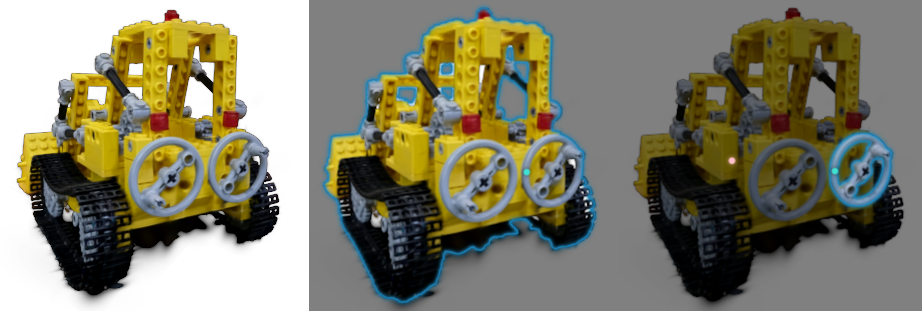
\includegraphics[width=\textwidth]{Images/samdemo.png}
	\caption{Illustration of SAM segmentation with point prompts. From left to right: the original LEGO bulldozer; SAM segmentation with a single positive point on the rear wheel, selecting the entire bulldozer; and SAM segmentation after adding a negative point on another part, isolating only the wheel.}
	\label{fig:samdemo}
\end{figure}
\FloatBarrier
\noindent
SAM achieves this by processing the input image through a vision transformer backbone, which encodes it into a high-dimensional feature representation. The user-provided prompts are embedded and integrated with these image features via a prompt encoder. A mask decoder then combines these elements to produce the final segmentation mask. This architecture allows SAM to leverage both spatial relationships and contextual information from the image, resulting in precise and adaptive segmentation that respects the user’s input constraints.
\subsection{SAGD}
SAGD (Segment Anything via Gaussian Decomposition) closely aligns with the goals of this thesis. It not only segments Gaussian Splats based on user input, typically in the form of a SAM-generated mask, but also smoothens the boundary by splitting splats that overlap the segmentation edge.
\\\\
The core process of SAGD begins with the user providing 2D prompts on one view of the scene. These prompts are mapped to their corresponding 3D Gaussians, which are then reprojected into multiple other views to identify the same splats from different perspectives. For each view, SAM is applied to generate a segmentation mask that reflects the user’s intent. Each Gaussian is then labeled based on a voting mechanism: if its projections consistently fall inside the masks across multiple views, it is included in the segment. To further improve the segmentation, SAGD employs Gaussian Decomposition at the segment boundary. This process splits overlapping splats into two parts—one included in the segment and the other excluded—producing a cleaner and more precise segmentation boundary. The final result is a segmentation of the Gaussian Splat that is both user-guided and geometrically refined.
\\\\
The authors of SAGD provide an open-source implementation of their method, which facilitates integration into this research. However, this implementation does not include its own test data. As a result, it was necessary to identify a suitable pre-trained scene for evaluation. Unlike the previous part of this thesis, this time the implementation required not only a \texttt{.ply} file containing the splats but also detailed information about the camera positions used to generate the Gaussian Splat. Conveniently, several scenes from the original Gaussian Splatting paper were available for download, complete with the required camera information. Unfortunately, the scene with the LEGO bulldozer was not among them. The criteria for selecting a scene remained consistent: it needed to be simple, clear, and easy to segment. Among the available options, the truck scene emerged as the most suitable choice, as illustrated in Figure~\ref{fig:truck_scene}. This scene was also used as an example in the SAGD paper itself.
\begin{figure}[h!]
	\centering
	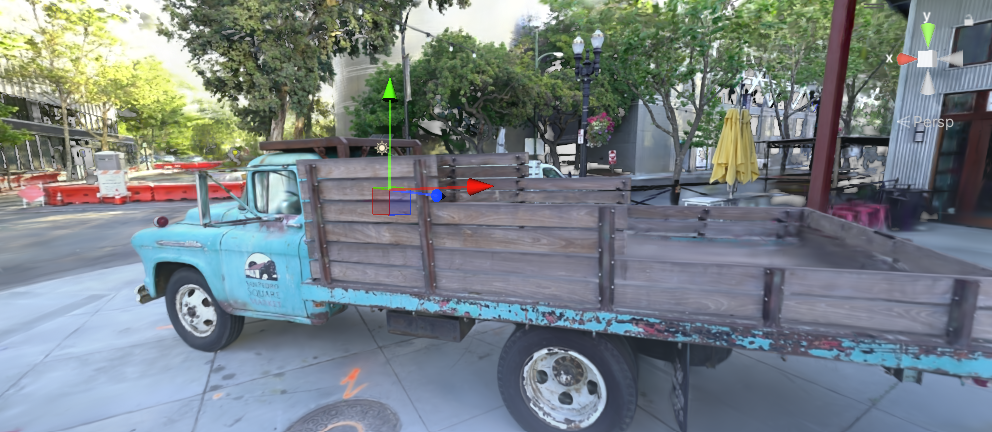
\includegraphics[width=\textwidth]{Images/truckscene.png}
	\caption{The truck scene, a pre-trained Gaussian Splat model used for segmentation testing. Rendered in Unity.}
	\label{fig:truck_scene}
\end{figure}
\FloatBarrier
\noindent
With a suitable scene now available, the SAGD implementation could be tested. The provided code is written in Python, specifically within a Jupyter notebook environment. To generate the image corresponding to each camera position, the implementation renders the Gaussian Splat from the perspective of each camera. This process is computationally intensive, as it must render for every camera position. Fortunately, the downloaded scene included the original images captured from these camera positions during the training of the splat data. Thus, in the notebook, an adaptation was made to load these pre-existing images in place of rendering new views, significantly reducing runtime. For validation, an image mask was recreated on the same frame as the example in the original SAGD paper. Initial testing focused on the projection step, examining how the system mapped the selected points into other views. This was achieved by displaying the masks generated for each view, as illustrated in Figure~\ref{fig:goodsagd} 
\begin{figure}[h!]
	\centering
	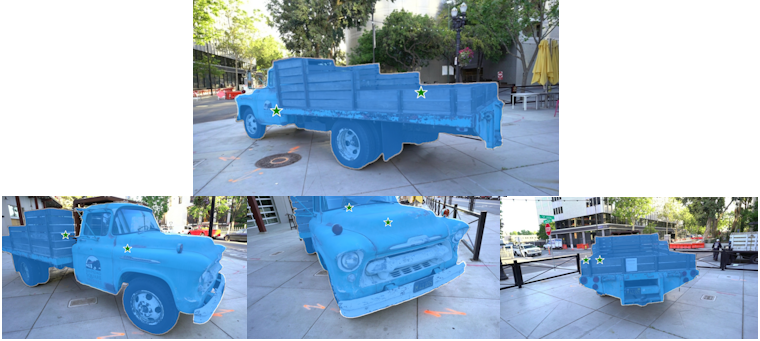
\includegraphics[width=\textwidth]{Images/goodsagd.png}
	\caption{Testing the SAGD implementation. Top: input image with two positive points provided to SAM and the corresponding segmentation mask. Bottom: three different camera viewpoints, each displaying the projected prompt-points and the mask generated by SAGD for that camera position, all correctly reflecting the intended segmentation.}
	\label{fig:goodsagd}
\end{figure}
\FloatBarrier
\noindent
With the recreated example from the paper showing promising results, additional input points were tested on the same frame. Specifically, the next test focused on evaluating how SAGD handles segmenting the wooden platform of the truck. However, this test revealed multiple issues, as illustrated in Figure~\ref{fig:issues}.
\begin{figure}[h!]
	\centering
	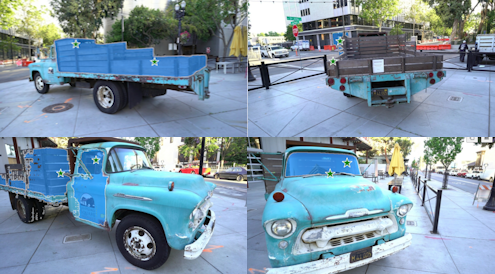
\includegraphics[width=\textwidth]{Images/badsagd.png}
	\caption{Testing the SAGD implementation. Top Left: input image with two positive points provided to SAM and the corresponding segmentation mask. The other three: three different camera viewpoints, each displaying the projected prompt-points and the mask generated by SAGD for that camera position. Notable issues with the segmentation are visible.}
	\label{fig:issues}
\end{figure}
\FloatBarrier
\noindent
First, it should be noted that the frames shown in Figure~\ref{fig:issues} have been selectively chosen to illustrate the limitations observed. While a substantial number of frames yielded correct segmentations, there were several additional frames beyond the three presented that displayed issues. These issues can be categorized into two core limitations of the implementation:
\begin{itemize}
	\item Convergence: In some cases, input points that are far apart in the original frame provide strong information for segmentation. However, under different viewing angles, these points may appear much closer together, reducing the specificity of the segmentation prompt. This convergence makes it more difficult for SAM to determine the intended segment, as observed in the top-right frame of Figure~\ref{fig:issues}. While this issue can be somewhat mitigated by adding additional positive points, it is possible for all available points to fall on the same plane in 3D space. In such cases, certain viewing angles may still cause clumping of the projected points, resulting in reduced prompt effectiveness.
	\item Occlusion: In the original frame, the input points are clearly located on a specific, unobstructed part of the object. However, when these points are projected into other views, changes in perspective or camera angle can cause parts of the object to become occluded by other elements of the scene. This means the projected points may land on areas of the image that visually correspond to different objects or regions, which SAM interprets as valid parts of the segment. As a result, the mask generated in these frames includes unintended areas. This issue is evident in the bottom two frames of Figure~\ref{fig:issues}. Notably, in this scenario, adding additional positive or negative points cannot resolve the issue. Regardless of the other prompts, SAM will consistently attempt to generate a mask that includes the incorrectly placed point due to its interpretation of the user’s intention.
\end{itemize}
Before exploring alternative methods of generating masks from other camera standpoints, it is both useful and logical to continue testing the remaining key components of SAGD: the voting system and the Gaussian Decomposition process. To evaluate these, the example will be revisited that was provided in the original SAGD paper—the segment that consistently produced accurate results. Figure~\ref{fig:sagdwithout} illustrates the output generated by the voting system alone, while Figure~\ref{fig:sagdwith} shows the same output after Gaussian Decomposition has been applied.
\begin{figure}[h!]
	\centering
	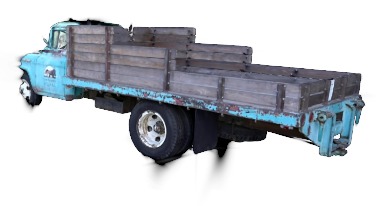
\includegraphics[width=0.9\textwidth]{Images/nodecomp.png}
	\caption{Result of applying SAGD on the example from the paper, without using Gaussian Decomposition. The segmentation is relatively clean, except for a missing portion at the front of the object.}
	\label{fig:sagdwithout}
\end{figure}
\begin{figure}[h!]
	\centering
	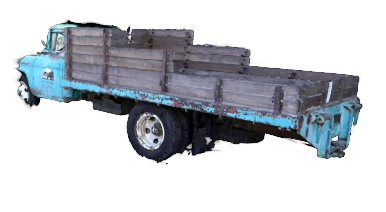
\includegraphics[width=0.9\textwidth]{Images/withdecomp.png}
	\caption{Result of applying SAGD on the example from the paper, with Gaussian Decomposition applied. The splats extending beyond the segment boundary at the bottom have been effectively removed. However, some additional minor errors have been introduced, such as a hole appearing in the black square behind the rear wheel.}
	\label{fig:sagdwith}
\end{figure}
\FloatBarrier
\noindent
The absence of the front of the truck in the segmentation is an undesirable outcome. While this issue is correctable, it will be addressed after the challenges identified earlier are resolved. Regarding the Gaussian Decomposition process, it performs its intended role of cleaning up boundary splats. The errors introduced are likely due to a combination of factors: imperfect initial segmentation data and the need for further fine-tuning of the decomposition frequency (as decomposition is not applied to every frame). However, refining this frequency is not a primary focus of this thesis.
\subsection{SAM2}
Throughout this section, it has been emphasized that an ideal implementation would accept a single SAM mask as input and automatically generate corresponding masks from different camera angles. This approach strikes an optimal balance between user control and automation: it enables the user to define a precise sub-object, while eliminating the need to manually create multiple masks from different perspectives—a process that would be nearly as cumbersome as the original method of extracting segments.
\\\\
To reiterate, the ideal algorithm would transform a single SAM mask into multiple masks from different angles, without encountering the same issues as the original SAGD projection approach. This approach would enable the user to define just one mask while allowing SAGD to propagate it into a complete segmentation across the Gaussian Splat. This process would ultimately result in a perfectly smooth separation of the subsegment from the rest of the scene.\\
During the exploration of methods to generate these additional 2D masks, a promising development was discovered through the SAM documentation: SAM2 \parencite{SAM2}. This extension of SAM introduces video segmentation capabilities. Its input structure is similar to that of image segmentation, with the key difference being that prompts can be placed on specific frames, guiding segmentation in those particular frames. SAM2 can then generalize these prompts to produce a segmentation mask for every frame in the video (see Figure~\ref{fig:children}).
\begin{figure}[h!]
	\centering
	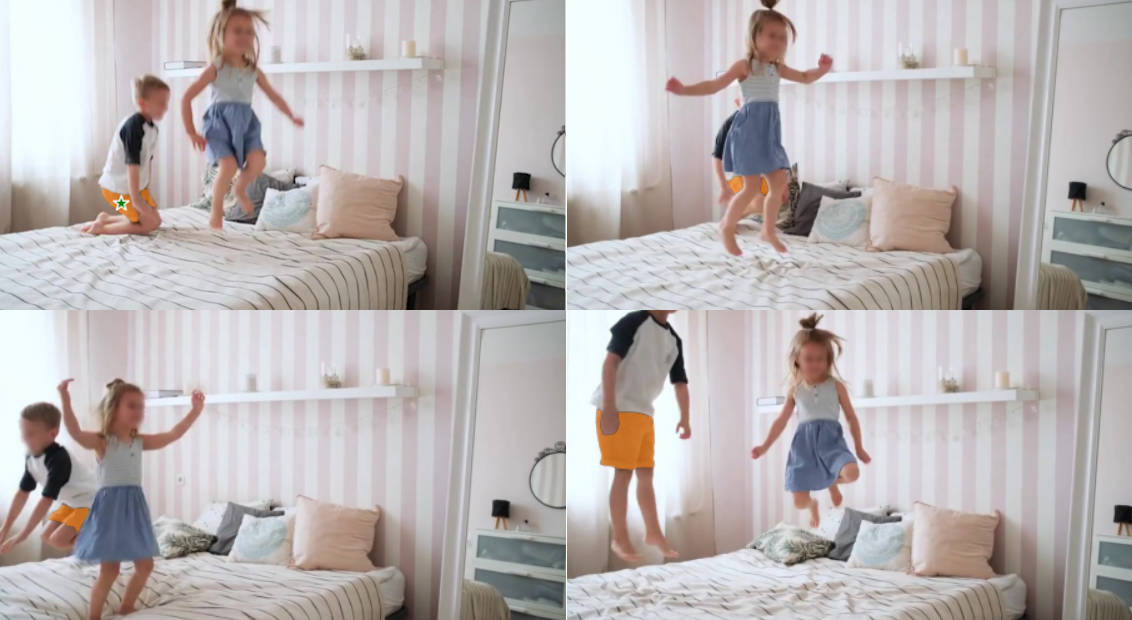
\includegraphics[width=\textwidth]{Images/children.png}
	\caption{Result of SAM2 on a sample video provided by the SAM2 repository. Top-left: input frame with a single positive prompt point and the generated segmentation mask. The remaining images show the masks generated by SAM2 on other frames of the video, illustrating the model's ability to propagate the segmentation across frames. Note that in the top-right frame, the pants are almost entirely obstructed, yet the model still returns the correct mask—highlighting a clear improvement over the occlusion issues encountered in the original SAGD algorithm.}
	\label{fig:children}
\end{figure}
\FloatBarrier
\noindent
SAM2 builds upon SAM’s image segmentation capabilities by extending them to video sequences. The user can provide segmentation prompts—such as points or bounding boxes—on any frame of the video. What sets SAM2 apart is its use of a memory mechanism that tracks and refines segmentation across frames. As the video progresses, SAM2 stores information from previous frames, including embeddings of both the frame features and the provided prompts. When processing a new frame, SAM2 retrieves this memory and integrates it with the current frame’s features to predict the segmentation mask. This enables SAM2 to maintain segmentation consistency even in the presence of occlusion, changes in object appearance, or movement.
\\\\
To leverage the capabilities of SAM2, it is necessary to provide a continuous sequence of frames as input. One theoretical approach to generate such a sequence involves defining a continuous camera path around the object, with the camera oriented toward the object, rendering each frame to a file, and recording the corresponding world position of the camera in a separate file. However, a more straightforward approach is often available: the images used to train the Gaussian Splat model are frequently captured as a continuous video sequence, rather than as a collection of images from random camera positions. When access to these training images is available, as is the case for the truck scene used in this project, the task of creating a continuous sequence of frames is effectively simplified. By using these ordered images directly as input for SAM2, the system can treat them as a continuous video sequence without additional processing. This approach was chosen as it provided a practical and efficient means to integrate SAM2, allowing the focus to remain on addressing the core issues of SAGD without introducing the additional overhead of generating synthetic sequences.
\\\\
To verify that the images form a continuous sequence, and to potentially aid in debugging, the separate images can be merged into a video by executing the following command in a Bash environment:
\begin{verbatim}
	ffmpeg -framerate 30 -i %06d.jpg -c:v mpeg4 -q:v 5 output.mp4
\end{verbatim}
The most straightforward approach to prompting a SAM2 video is to begin with the first frame and incrementally add positive and negative points to that frame until the generated mask closely aligns with the intended segment. However, SAM2 is not without its limitations. Due to its more sophisticated architecture compared to standard SAM, a greater number of points may be required to obtain a satisfactory mask for the first frame alone (see Figure~\ref{fig:sam2struggle}). Furthermore, while the masks generated for most frames may be acceptable, certain frames can still produce entirely inaccurate segmentations (see Figure~\ref{fig:sam2adapt}). Unlike the projection-related issues encountered in SAGD, these problems can generally be resolved by adding more input points—either to the initial frame or directly to the problematic frames.
\begin{figure}[h!]
	\centering
	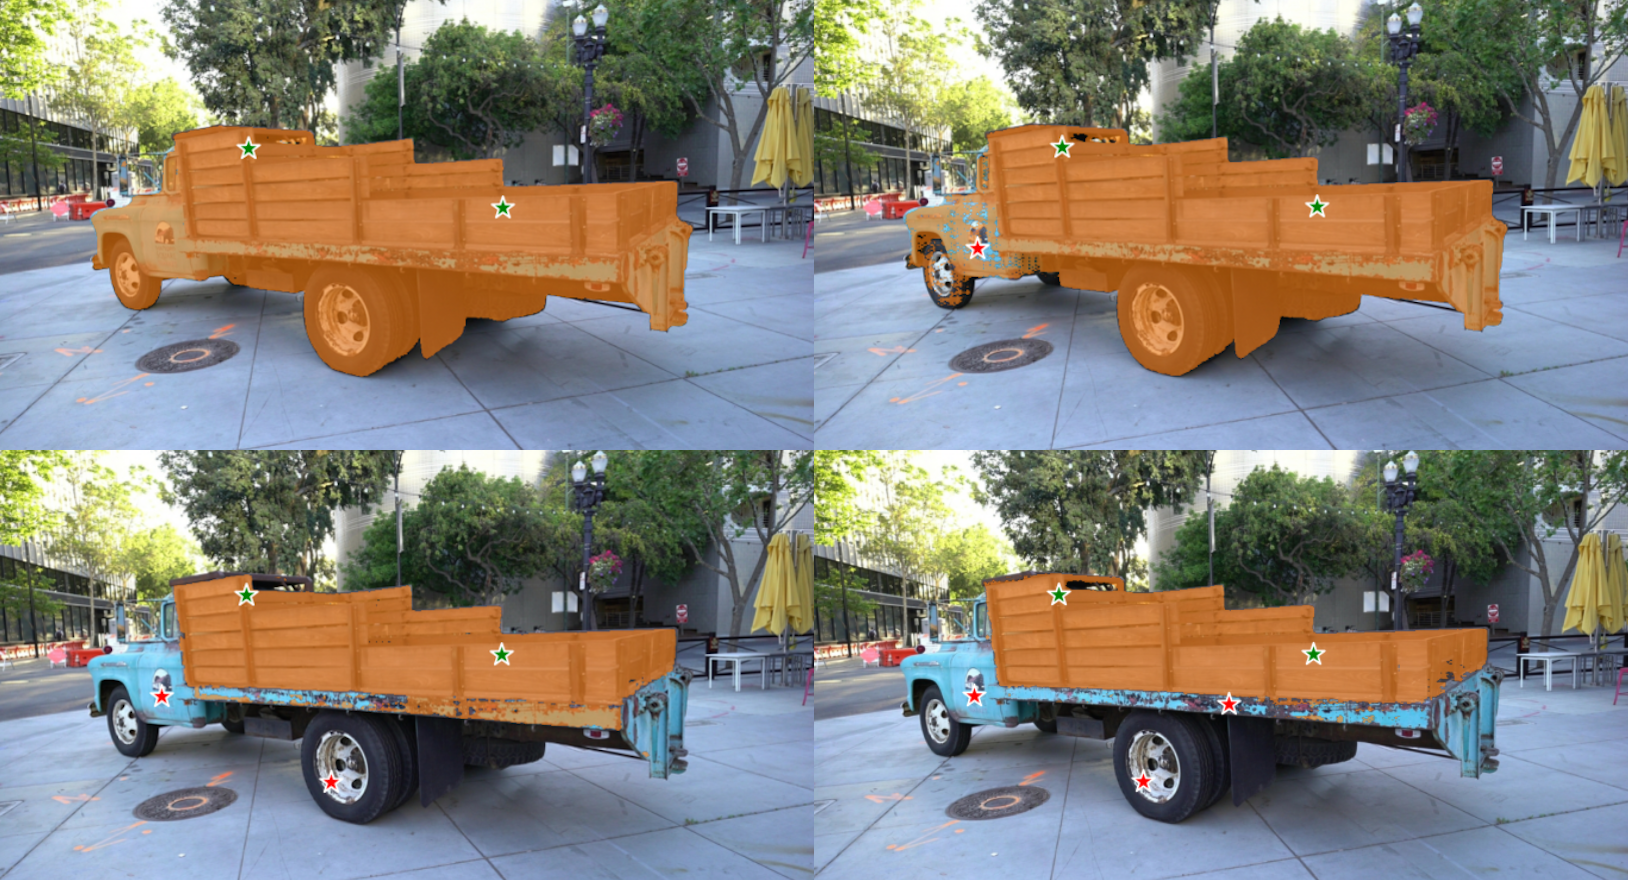
\includegraphics[width=\textwidth]{Images/sam2struggle.png}
	\caption{Progress of prompting the first frame in SAM2 to segment the wooden platform. Top-left: initial mask generated with two positive points. Subsequent images illustrate the addition of negative points, progressively refining the mask. The final frame (bottom-right) shows a mask that, while not perfect, achieves a satisfactory result across the video.}
	\label{fig:sam2struggle}
\end{figure}
\begin{figure}[h!]
	\centering
	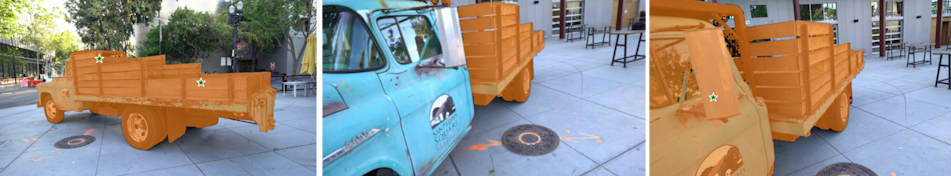
\includegraphics[width=\textwidth]{Images/sam2adapt.png}
	\caption{Segmentation of the entire truck using SAM2. Left: initial mask generated with only two positive points. Middle: a frame where the front of the truck is excluded from the mask due to its absence in some frames. Right: adding a single additional positive point to the problematic frame effectively resolves the issue.}
	\label{fig:sam2adapt}
\end{figure}
\FloatBarrier
\noindent
SAM2’s advantage lies in its ability to maintain temporal consistency and integrate contextual information from both the prompts and the sequence of frames. This enables it to produce reliable masks across the video with minimal additional input, contrasting with projection-based approaches where prompt points can easily shift to unrelated areas. As a result, the number of supplementary points required per segment remains limited, keeping the process significantly more efficient and user-friendly than manual segmentation or per-frame projection methods.
\\\\
To demonstrate the reliability of SAM2, Figures~\ref{fig:sam2whole} and~\ref{fig:sam2wood} replicate the same experiment conducted with the projection-based approach. Starting from the same mask (requiring slightly more prompt points), the same frames were inspected. While some degree of selective framing has been used to highlight the contrast more effectively, it is important to note that any frame yielding an incorrect mask can be readily corrected by adding additional prompts.
\begin{figure}[h!]
	\centering
	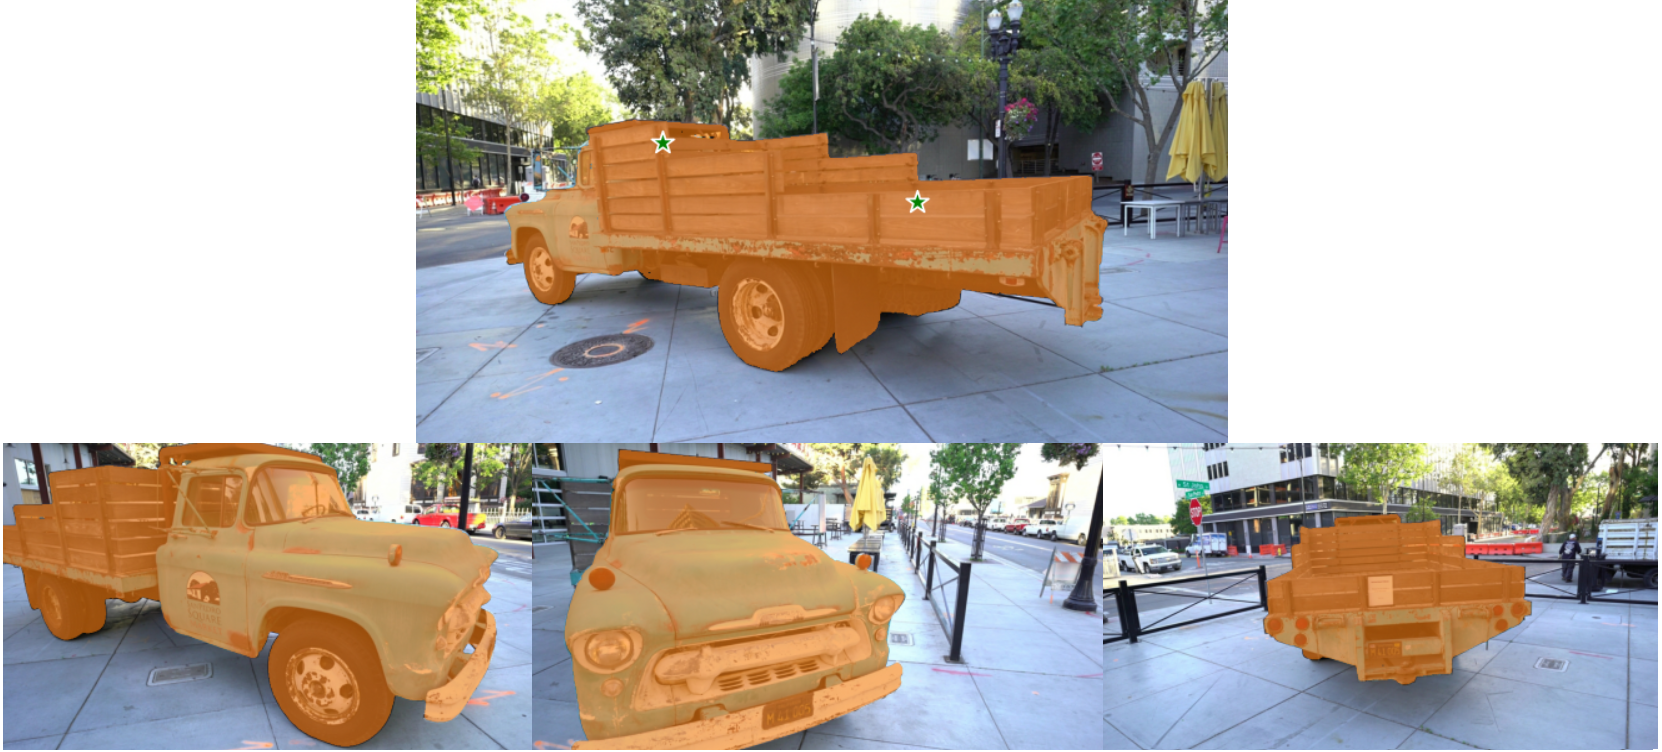
\includegraphics[width=\textwidth]{Images/sam2whole.png}
	\caption{Replication of the experiment from Figure~\ref{fig:goodsagd}, using SAM2 instead of projection.}
	\label{fig:sam2whole}
\end{figure}
\begin{figure}[h!]
	\centering
	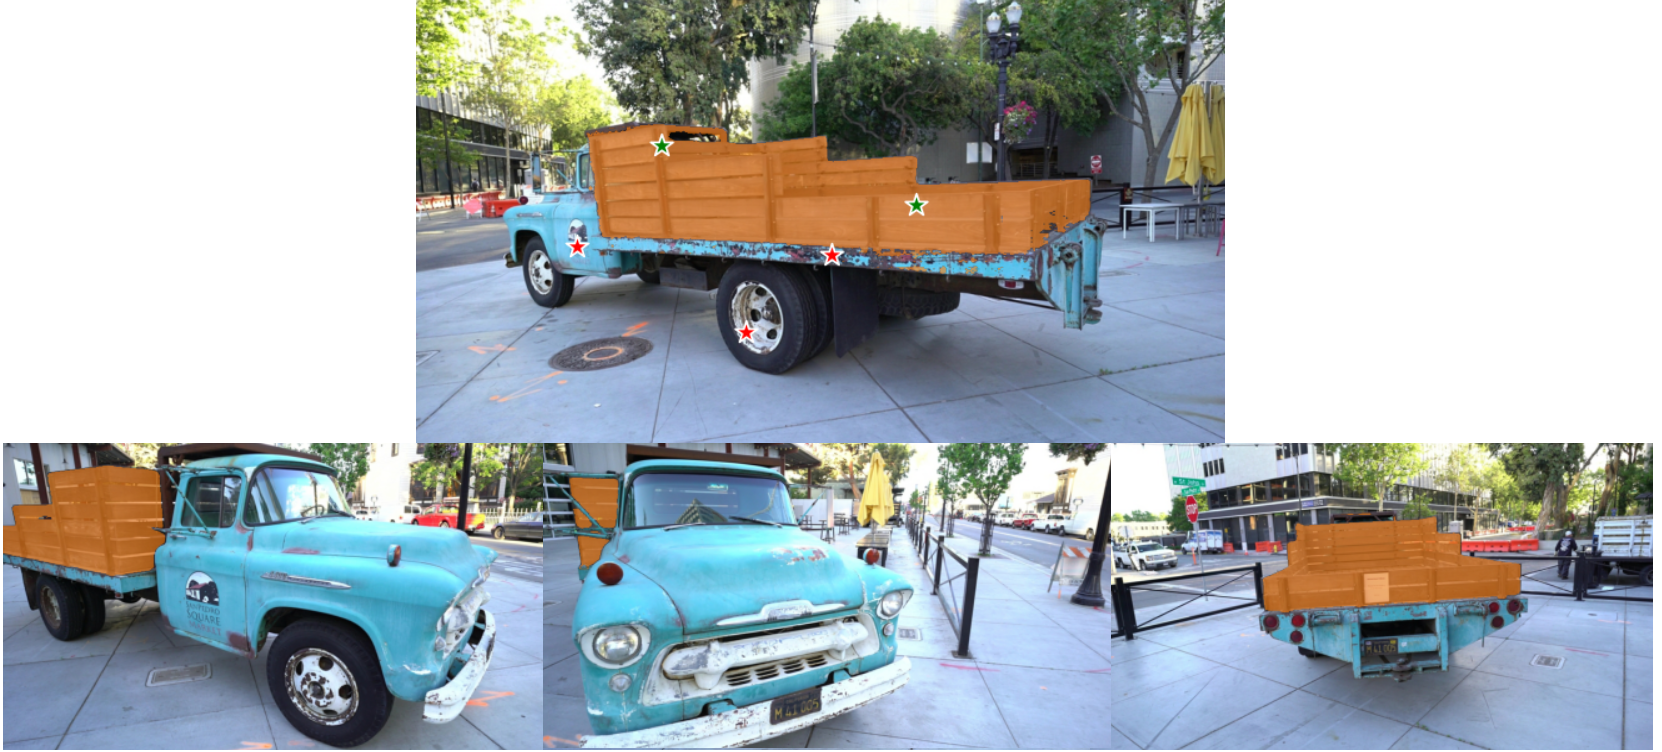
\includegraphics[width=\textwidth]{Images/sam2wood.png}
	\caption{Replication of the experiment from Figure~\ref{fig:issues}, using SAM2 instead of projection.}
	\label{fig:sam2wood}
\end{figure}
\FloatBarrier
\noindent
Having demonstrated the potential of SAM2 to produce consistent and efficient segmentation masks across multiple viewing angles, the next logical step was to integrate these results with the SAGD pipeline. Instead of relying on per-frame projection methods to generate masks, the output of SAM2 was leveraged directly. To facilitate this integration and streamline debugging, the generated masks were serialized into a pickle file—a standard Python format for storing and retrieving data structures such as dictionaries. In this case, the pickle file contained a mapping from each frame index to its corresponding segmentation mask. The SAGD implementation was then modified to read this file and use the precomputed masks as input for its downstream processing stages.\\\\
To validate this approach, the Gaussian Splat of the wooden platform was extracted using the same prompt points as in the earlier example. The resulting segmentation is illustrated in Figure~\ref{fig:sagdwoodply}.
\begin{figure}[h!]
	\centering
	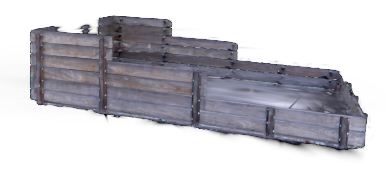
\includegraphics[width=\textwidth]{Images/sagdwoodply.png}
	\caption{Resulting Gaussian Splat of the wooden platform, generated using SAM2-based masks as input for the SAGD pipeline. The extracted segment accurately captures the platform’s structure while excluding surrounding elements, illustrating the reliability of SAM2-generated masks for segmentation tasks.
	}
	\label{fig:sagdwoodply}
\end{figure}
\FloatBarrier
\noindent
\subsection{Hierarchy}
While the separation of a single segment is advantageous, the intended use case of this thesis involves interactive applications where both the subsegment and its parent object must coexist within the scene. Therefore, it is necessary to implement an intuitive and efficient method for segmenting a subcomponent while retaining both the isolated segment and the remainder of the object as distinct, non-overlapping entities.
\\\\
The process of first segmenting the wooden platform of the truck and then performing a separate segmentation of the truck without the platform is not only impractical, but also prone to errors. This approach introduces the risk of including certain splats in both segments, resulting in incorrect visual artifacts. A hierarchical segmentation method, which preserves a clear parent-child relationship between the segments, is thus essential for maintaining both visual fidelity and workflow efficiency.
\\\\
The most straightforward approach to achieve hierarchical segmentation, while also providing maximal control to the user, is to employ a layered data structure. Specifically, this thesis defines the following recursive structure:
\begin{lstlisting}[tabsize=2,caption=Definition of the recursive data structure used to represent hierarchical segmentation prompts and their relationships in SAM2, label=code:recursivedata,breaklines=true,breakatwhitespace=true,basicstyle=\ttfamily\footnotesize]
@dataclass
class framePrompt:
	points: np.ndarray
	labels: np.ndarray
	frame_number: int

@dataclass
class LayeredMaskPrompt:
	frameprompts: list[framePrompt]
	subobjects: list['LayeredMaskPrompt']
\end{lstlisting}
This structure enables the user to define high-level parent objects, using SAM2 prompt points and labels, and to specify subordinate child objects by nesting additional LayeredMaskPrompt entries. This recursive arrangement naturally supports hierarchical parent-child relationships, allowing for flexible and precise segmentation.
\\
To compute the segmentation masks for each frame, SAM2 processes this hierarchical prompt structure and generates frame-wise masks for each node in the hierarchy. These masks are stored in a similarly recursive format using a pickle file: each dictionary contains a masks key, holding the mask information for the respective frames, and a subobjects key containing a list of child dictionaries structured identically.
\\\\
SAGD can directly process these recursive structures to generate the desired segmentation. To ensure that splats do not appear redundantly in both parent and child segments—and to enforce a clean hierarchical split—the algorithm operates recursively. First, for a given node in the hierarchy, it computes the mask over the 3D splats of the object using standard techniques. It then iterates over each subobject (child node), invoking the same recursive procedure on each. Each recursive call returns the complete set of splats associated with the child, regardless of whether those splats are unique to the child or shared with its descendants. The parent node aggregates these returned splat sets to identify which of its own splats have been claimed by its subobjects. After processing all children, the parent writes to the output PLY file only those splats that were not claimed by any child, ensuring exclusivity. Finally, the parent returns the complete set of splats assigned to itself—including those shared with its subobjects—allowing this information to propagate upward through the recursion.
\\\\
While this approach offers substantial control to the user, it also places significant responsibility on them to ensure that the defined hierarchy is coherent and meaningful. For instance, the user could define two entirely separate nodes with substantial overlap in their segmentation regions, resulting in duplicated splats in the overlapping areas. However, due to the intuitive interface and real-time visual feedback provided by SAM2, the risk of such errors can be mitigated without imposing a significant burden on the user.
\\\\
To validate the correctness of the new hierarchical algorithm, a straightforward test configuration was devised: two prompts were defined—one describing the entire truck and one describing the wooden platform. The platform prompt was specified as a child node of the truck prompt, both utilizing the same prompt points as in the earlier experiments. The resulting segmentation is illustrated in Figure~\ref{fig:woodpair}.
\begin{figure}[h!]
	\centering
	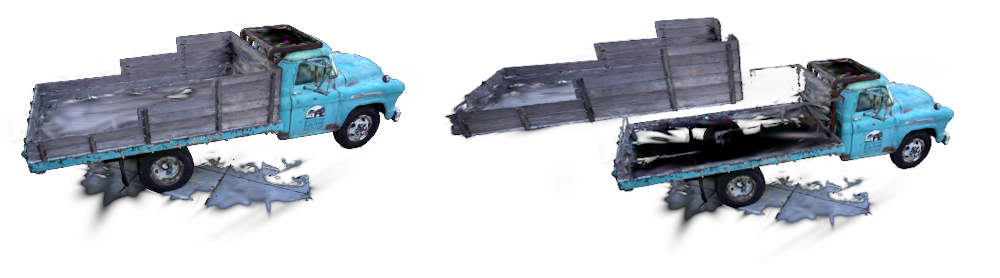
\includegraphics[width=\textwidth]{Images/woodpair.png}
	\caption{Hierarchical segmentation of the truck and wooden platform. Left: both segments are shown in their original positions, appearing as a single cohesive object. Right: the wooden platform has been translated slightly to visually demonstrate its separation from the truck and to highlight the precision of the segmentation. Notable artifacts include small areas where the wood remains connected to the truck—likely due to minor segmentation inaccuracies in SAM2—and holes in the truck where the platform was extracted, resulting from missing splat data in occluded regions and the platform’s thin structure.
	}
	\label{fig:woodpair}
\end{figure}
\FloatBarrier
\noindent
\subsection{Multimask Automation}
This section has explored the challenge of balancing user control with automation in the segmentation process. While the previously described hierarchical method offers extensive flexibility, it also places a considerable burden on the user to maintain logical consistency, particularly when defining complex hierarchies. In certain cases, it may be desirable to reduce user intervention, especially when the relationship between segments is sufficiently straightforward and can be inferred from the context of the object and scene. This motivates the search for a method that requires the user to annotate only a single segment, while automating the determination of hierarchical relationships, thereby simplifying the segmentation process without sacrificing accuracy.
\\\\
Once again, the key enabler of this approach is SAM itself. During image segmentation, SAM provides an optional parameter, \texttt{multimask\_output}, which, when set to true, instructs the model to generate multiple segmentation masks instead of a single one. Specifically, it returns three masks, each representing a different level of segmentation granularity (see Figure~\ref{fig:multidemo}). These masks are hierarchically nested, with each smaller mask fully contained within the next larger one, effectively creating a parent-child relationship. Additionally, each mask is accompanied by a confidence score, providing an automated means to evaluate the quality of the segmentation proposals and to filter out suboptimal candidates.
\begin{figure}[h!]
	\centering
	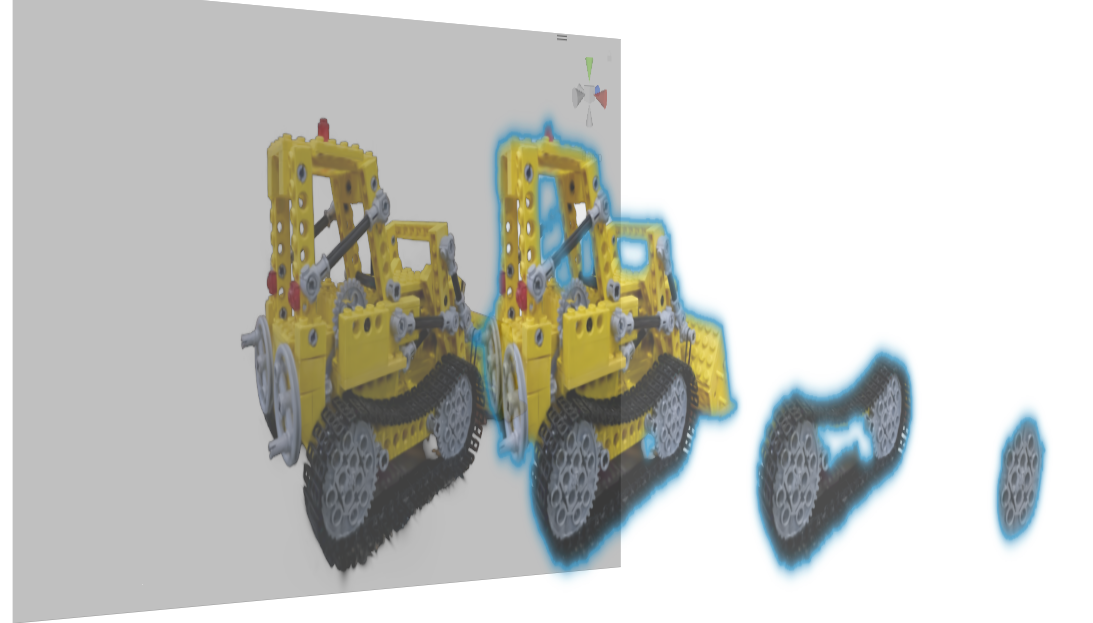
\includegraphics[width=\textwidth]{Images/multidemo.png}
	\caption{Demonstration of SAM’s multimask segmentation functionality on the LEGO bulldozer model. A single wheel was selected as the initial segment, resulting in three hierarchical masks: the smallest corresponds to the wheel itself, followed by the caterpillar tracks, and finally the entire bulldozer as the largest segment.
	}
	\label{fig:multidemo}
\end{figure}
\FloatBarrier
\noindent
It is important to note that the \texttt{multimask\_output} functionality is available only for image segmentation, not for video segmentation, which is the mode required for this project. However, video segmentation in SAM2 introduces an alternative feature that had not been utilized previously: in addition to providing prompts in the form of points or bounding boxes on a specific frame, the user can supply a full mask as input for that frame. This capability enables the following pipeline, as implemented in this thesis:
\\
The user provides standard prompt points to define a target segment, from which the image segmentation algorithm generates three hierarchical masks. Applying a simple filter based on the quality scores of these masks, only the most confident masks are retained. This produces a local hierarchy of the segment. Each of these confident masks is then used as an input prompt for video segmentation, resulting in corresponding masks for each frame in the video. The output data is then stored using the recursive data structure described in the previous section, with the hierarchical relationships already established by the multimask output. From this point onward, SAGD processes the input exactly as before, requiring no further modifications to the segmentation or rendering pipeline.
\\\\
However, during the implementation and experimentation with various \linebreak prompts and configurations, it became apparent that the original SAM provided superior results for image segmentation compared to SAM2. This was particularly evident when using the \texttt{multimask\_output} functionality, as demonstrated in Figure~\ref{fig:sam1better}. Consequently, despite SAM2’s integrated image segmentation capabilities, the pipeline was adjusted to maximize segmentation quality: the user provides prompt points, which are processed by the original SAM image segmentation to generate three hierarchical masks. These masks are then filtered based on confidence scores and subsequently used as input for the SAM2 video segmentation component. The resulting hierarchical masks are then processed by SAGD, which generates the final segmented Gaussian Splat. In effect, this approach integrates three distinct tools—SAM, SAM2, and SAGD—into a single pipeline to achieve optimal results.
\begin{figure}[h!]
	\centering
	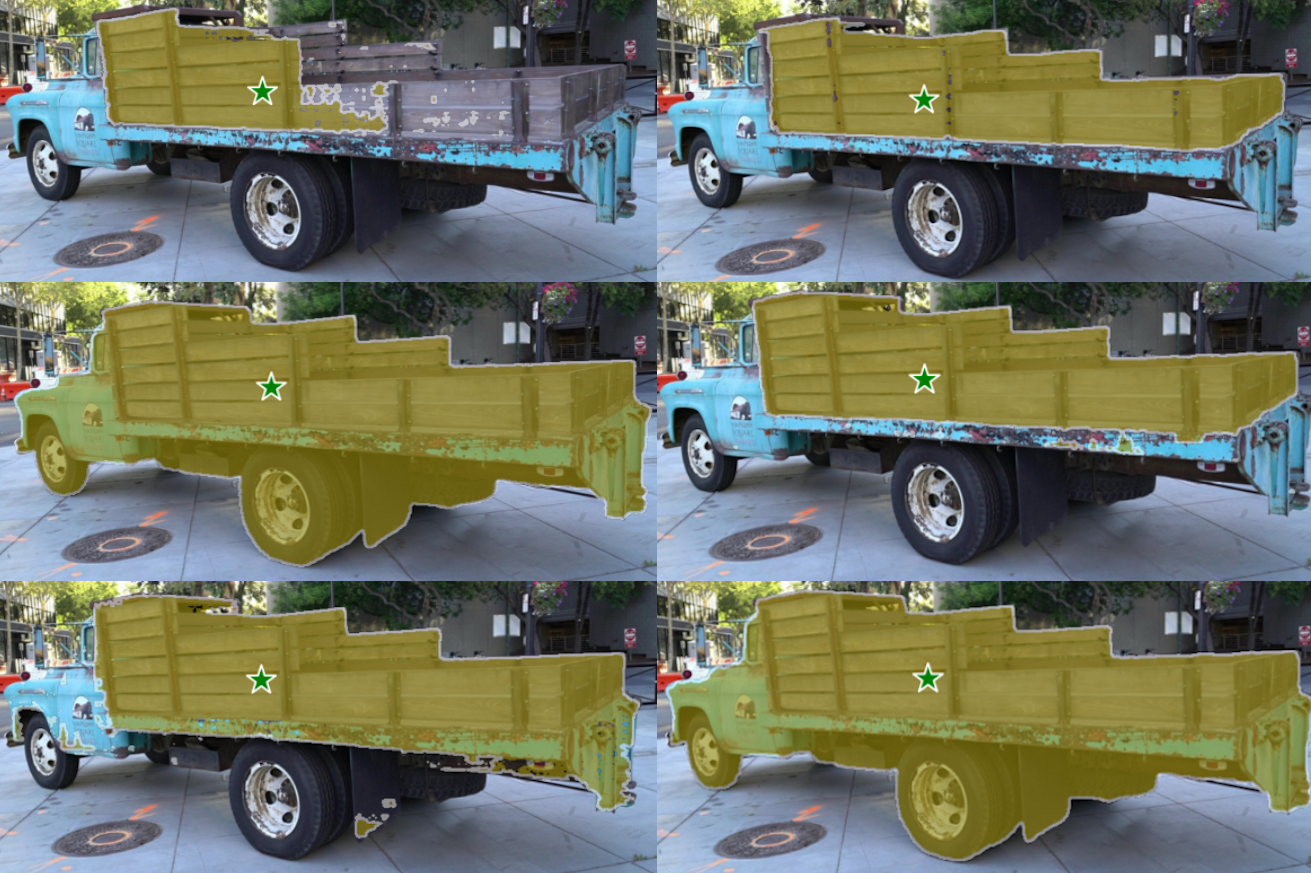
\includegraphics[width=\textwidth]{Images/sam1v2.png}
	\caption{Comparison of multimask output from SAM2 (left column) and original SAM (right column) for the same input prompt. Each row corresponds to one of the three hierarchical masks generated by the respective model. Despite identical input, SAM2 consistently fails to accurately segment the wooden platform as a distinct region, whereas SAM demonstrates clearer separation.
	}
	\label{fig:sam1better}
\end{figure}
\FloatBarrier
\noindent
As with all previous implementations, the new pipeline was tested on the same objects. Notably, this iteration required significantly less user input: due to the enhanced automation provided by the multimask segmentation approach, only a single positive prompt point was necessary to define the wooden platform and its hierarchical relationship with the truck, compared to the seven points required in the previous section. The resulting segmentation is illustrated in Figure~\ref{fig:multipair}.
\begin{figure}[h!]
	\centering
	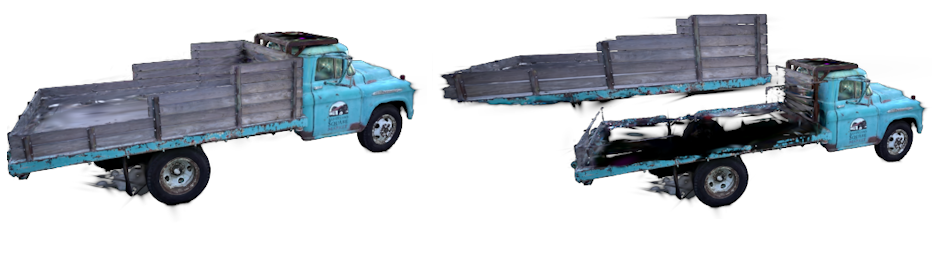
\includegraphics[width=\textwidth]{Images/multipair.png}
	\caption{Result of the semi-automated multimask segmentation pipeline applied to the wooden platform and truck. The outcome closely resembles the segmentation achieved with full user control. The primary difference is the erroneous inclusion of a portion of the truck's blue frame in the wooden segment. Nonetheless, considering the substantial reduction in user input required, the overall result remains highly effective.
	}
	\label{fig:multipair}
\end{figure}
\FloatBarrier
\noindent
It is important to note that this tool is applicable only under specific criteria and is not intended to replace the simple hierarchical segmentation algorithm. Rather, it serves as a complementary tool, best suited for clear and pronounced segments where its automated approach can be effectively leveraged. In contrast, the hierarchical algorithm remains essential for handling more complex cases that require finer user control. This dual strategy ensures that, in the worst-case scenario, a user-friendly implementation is always available, while in the best case, segmentation can be achieved with minimal user effort.
\subsection{Full Automation}
As stated in the related work section, the primary focus of this part has been on user-guided segmentation, rather than fully automated approaches. However, as the developments progressed and the combination of SAM, SAM2, and SAGD matured, it became increasingly compelling to explore the extent to which these tools could be leveraged to approach full automation. If it were possible to identify all potential segments within a single frame, then the multimask output functionality, combined with video segmentation and SAGD, could be employed to propagate these segments throughout the video and generate the complete Gaussian Splat segmentation automatically.
\\\\
For the final time, SAM provides a suitable solution through its automatic mask generation functionality. This feature leverages a grid-based approach to systematically generate segmentation masks for the entire image. Specifically, it places a series of positive prompt points across a grid spanning the image, and for each prompt point, it generates a corresponding mask. These masks effectively partition the image into distinct segments, essentially fracturing the scene into its constituent parts (see Figure~\ref{fig:everything}).
\begin{figure}[h!]
	\centering
	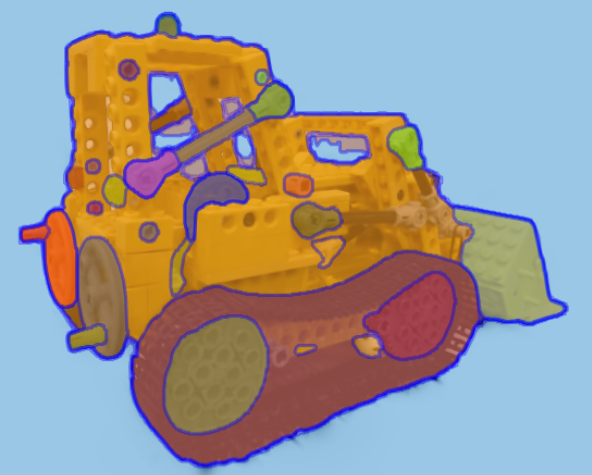
\includegraphics[width=0.6\textwidth]{Images/everything.png}
	\caption{Segmentation of the LEGO bulldozer using SAM’s automatic mask generation functionality. The image illustrates the resulting distinct masks, each rendered in a different color, effectively partitioning the scene into separate segments.
	}
	\label{fig:everything}
\end{figure}
\FloatBarrier
\noindent
While this automatic mask generation provides an effective means of detecting all segments within a frame, masks as output format present certain challenges. Specifically, the multimask functionality cannot take a mask as input, which is essential for determining the underlying hierarchy and identifying how individual segments combine into larger parent segments. However, the automatic mask generation output includes not only the segmentation masks themselves, but also the specific point prompt that generated each mask. As a result, the masks themselves can be discarded, and what remains is a minimal set of point prompts that each define a unique segment. By applying the algorithm described in the previous section, each of these points can be expanded into a hierarchical set of segments. This approach brings the thesis close to achieving a fully segmented 3D Gaussian Splat with minimal user intervention.
\\\\
The primary limitation preventing fully automated segmentation at this stage is that the current processes operate in isolation; they do not interact or merge hierarchies. When multiple segments share overlapping or similar parent regions, many splats are duplicated across different outputs. To address this, it is necessary to consolidate all segments and their hierarchies into a single, cohesive structure. The most effective solution is to discard the parent-child relationships introduced by the multimask segmentation and instead compile all multimasks that exceed a certain quality threshold into a single list. This adjustment is essential because complex interactions between segments can introduce inconsistencies in the hierarchy, particularly when additional overlapping segments were not initially detected.
\\\\
Once all masks are consolidated into a list, duplicates can be effectively filtered out. The simplest approach is to iterate through the list and construct a second list of unique masks. To determine whether a mask is unique, it is compared against all masks already present in the unique list. This comparison is based on the Intersection over Union (IoU) metric, which calculates the ratio of the overlapping area between two masks to their combined area. By using IoU, even masks that are nearly identical except for minor pixel differences can be identified as duplicates and removed
\\\\
Finally, the parent-child relationships can be re-established from the ground up and stored in a recursive data structure. To construct this structure, the set of unique masks is first sorted from largest to smallest based on their size. The algorithm then iterates through this sorted list, assigning each mask as the child of the smallest mask that fully contains it. If no such enclosing mask exists, the mask is designated as a root segment without a parent. To determine containment, the algorithm calculates the ratio of the overlap area between two masks to the area of the smaller mask, ensuring that minor differences or outlier pixels do not disrupt the hierarchical assignment. At the end of the iteration, a complete recursive hierarchical structure is formed. The same recursive algorithm described in the previous section can then be applied seamlessly, generating video segmentations for each mask and ultimately producing the final Gaussian Splat segmentation.
\\\\
A final practical challenge emerged: the data structure was too large to fit within a single pickle dump file. To resolve this, the recursive hierarchical structure was emulated using a folder-based system. Each folder corresponds to a segment, containing a pickle file with its frame masks and a series of subfolders representing its child segments. SAGD processes this structure by traversing the folders and loading each pickle file individually. This approach effectively preserves the hierarchical segmentation while circumventing the limitations of the pickle format.
\\\\
With a large number of PLY files now generated for the hierarchical segments, it became necessary to extend the Unity extension by introducing a tool to automatically load these hierarchical PLY files. To enable the Unity code to recognize and reconstruct the hierarchy, the same folder-based approach described previously was adopted: each folder contains a single PLY file and a set of subfolders representing its subsegments. The new tool operates similarly to the existing PLY loader, but with key differences. Specifically, it traverses the entire folder structure, handles multiple PLY files simultaneously, and creates corresponding GameObjects in Unity with the appropriate PLY assets assigned. Moreover, it establishes the correct parent-child relationships among the GameObjects, based on the hierarchy inferred from the folder structure. This design enables the complete hierarchical scene to be loaded into Unity with a single operation.
\\\\
As with the previous sections, the final implementation was tested using the established scene, focusing on the first frame as a reference point. The setup remained consistent with earlier experiments, allowing for a direct comparison of the results achieved with the full automation approach. The resulting segmentation is illustrated in Figure~\ref{fig:truckparts} and Figure~\ref{fig:best}.
\begin{figure}[h!]
	\centering
	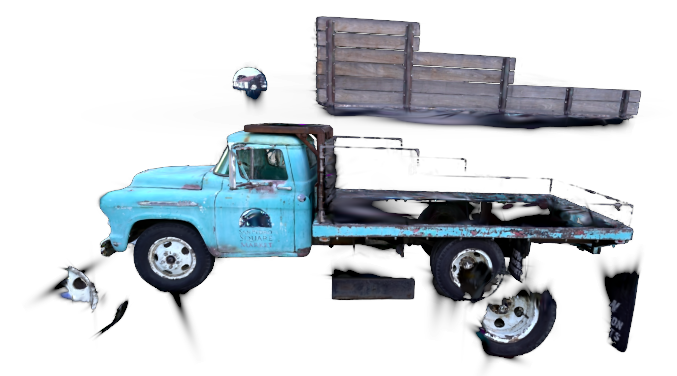
\includegraphics[width=\textwidth]{Images/truckparts.png}
	\caption{Exploded view of the truck’s segmentation, highlighting separated components for evaluation.}
	\label{fig:truckparts}
\end{figure}
\begin{figure}[h!]
	\centering
	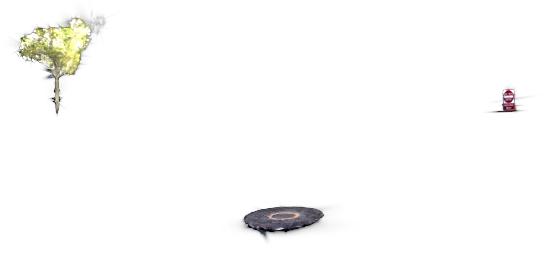
\includegraphics[width=\textwidth]{Images/best.png}
	\caption{A selection of non-truck segments extracted from the scene, illustrating examples of successful segmentation.}
	\label{fig:best}
\end{figure}
\FloatBarrier
\noindent
While some segments were successfully extracted, an equal or greater number were found to be incomplete or incorrect, often representing only a small fraction of the intended object. This limitation is likely due to challenges in the voting system used to consolidate video segmentation masks into a single splat representation. Specifically, this system appears to struggle with handling occlusions and off-screen regions, which can lead to incomplete or fragmented segmentations. Despite these challenges, the automation approach remains a notable achievement. It demonstrates the full integration and utilization of SAM and SAM2 capabilities, achieving meaningful segmentation of several objects from an initially unsegmented scene. It is important to emphasize that users seeking more consistent and reliable segmentation results should consider the multimask approach or the recursive hierarchical method. These algorithms are designed to complement each other, offering flexibility depending on the segmentation requirements and complexity of the scene.
\subsection{Conclusion}
This section has demonstrated the evolution of segmentation techniques for Gaussian splatting, culminating in a system that balances user-guided input with varying levels of automation. Beginning with manual prompt-based segmentation, the work progressed through hierarchical segmentation using multimask outputs, and finally approached full automation with SAM’s automatic mask generation capabilities. Each stage built upon the previous, incrementally reducing the manual effort required while simultaneously expanding the scope and complexity of segmentable scenes.
\\
The segmentation strategies developed throughout this section illustrate both the strengths and limitations of current techniques. While full automation shows promise, it still faces challenges such as managing overlapping segments and inconsistencies in mask hierarchies. However, by offering a range of methods—from manual to semi-automated to fully automated—the pipeline provides a flexible and practical toolkit adaptable to various scene complexities and user needs. The tools and approaches developed here establish a solid foundation for preparing complex splat-based scenes for animation and further processing.
\section{Future Work}
While the rendering improvements introduced in this thesis successfully addressed key challenges, there remains potential for further streamlining and optimization. However, as these rendering changes do not present immediate obstacles to the functionality of the system, they have not been identified as a priority for future exploration.\\\\
In contrast, segmentation continues to be a rich and open area for further research and development. Several promising directions could be pursued. One possibility involves implementing an automated camera system in Unity that dynamically captures multiple perspectives of an object, enabling segmentation of Gaussian splats even in the absence of the original training camera data.\\
Another avenue lies in refining the current voting system, which consolidates per-frame segmentation results but struggles with occlusion and incomplete visibility. Investigating alternative voting mechanisms or occlusion-aware strategies could significantly enhance segmentation robustness.
\\\\
Additionally, there is considerable potential in exploring more advanced, hybrid approaches that integrate both image-based and geometric information. The current pipeline relies heavily on two-dimensional prompting and mask generation, yet the inherent properties of splats—such as position, size, orientation, and color—offer valuable cues that remain underutilized. Developing algorithms that fuse these geometric attributes with traditional image segmentation techniques could unlock more precise and comprehensive segmentation capabilities, further advancing the field.
\section{Conclusion}
This thesis has explored the challenges and possibilities of working with Gaussian splats, focusing on two primary aspects: rendering improvements and segmentation strategies. The research question posed whether global per-splat sorting is essential to achieve acceptable rendering quality in Gaussian splatting, and whether it can be effectively implemented in Unity. The corresponding hypothesis suggested that global per-splat sorting might not be strictly necessary but could be implemented if required. The findings of this thesis, however, demonstrate that global per-splat sorting is indeed essential to resolve rendering artifacts, thereby disproving the initial assumption. Nevertheless, the hypothesis regarding implementation was confirmed, as a global per-splat sorting approach was successfully developed and integrated into Unity, achieving the desired improvements in rendering quality.

On the segmentation front, a progressive approach was adopted, beginning with manual prompt-based methods and culminating in a near-fully automated pipeline leveraging the capabilities of SAM, SAM2, and SAGD. The integration of hierarchical and multimask segmentation techniques demonstrated the potential for both fine control and increased efficiency. This supports the hypothesis that semi-automatic segmentation methods can reduce manual input requirements while maintaining, and in certain cases enhancing, segmentation accuracy. However, the results also revealed the inherent complexities and limitations of current systems, particularly in handling occlusion and building robust segment hierarchies.

Although challenges remain, the contributions of this thesis provide a strong foundation for future work. By offering both practical tools and conceptual frameworks, it paves the way for continued development in the segmentation and rendering of Gaussian splats, with potential applications in interactive graphics, animation, and beyond.
\FloatBarrier\addcontentsline{toc}{section}{References}
\noindent\printbibliography
\end{document}
